%\documentclass[handout]{beamer}
%\usepackage{pgfpages}
%\pgfpagesuselayout{4 on 1}[a4paper, landscape, border shrink=5mm]
%\pgfpageslogicalpageoptions{1}{border code=\pgfusepath{stroke}}
%\pgfpageslogicalpageoptions{2}{border code=\pgfusepath{stroke}}
%\pgfpageslogicalpageoptions{3}{border code=\pgfusepath{stroke}}
%\pgfpageslogicalpageoptions{4}{border code=\pgfusepath{stroke}}
\documentclass[10pt]{beamer}
%\usetheme{nesl}  % Now it's a beamer presentation with the NESL theme!
\usetheme{Warsaw}
\usecolortheme{default}
\usepackage{tikz}
\usetikzlibrary{shapes,arrows}
\usepackage{url}
\usepackage{movie15}
\usepackage{verbatim}
\usefonttheme{serif}
\usepackage{fancybox}
\beamersetuncovermixins{\opaqueness<1>{25}}{\opaqueness<2->{15}}

% Make a new command that will make a new subsection and a frame with the same title
\newcommand{\fst}[2]{\subsection{#1}\frame{\frametitle{#1} #2}}

% Standard LaTeX stuff - note the optional abbreviated title being provided
\title{Development of regional GSI-based \\ WRF 4D-Var}
\author[Zhang and Huang]{Xin Zhang \and Xiang-Yu Huang}

\date{~\\
~\\ \tiny{June 28 2011, GSI Workshop, Boulder, CO}\\
  ~\\
   ~\\
 \tiny{NCAR is sponsored by the National Science Foundation}
}

\institute[NCAR Earth System Laboratory]{
% \url{xinzhang@ucar.edu} \\
   NCAR Earth System Laboratory \\
%  \url{ook@ucw.cz}\\
%  Charles University, Prague
}

% We want the NSF department logo
%\logo{
\includegraphics[height=.5in]{nsf1.jpg}}
\logo{
\includegraphics[height=.25in]{NSF_NESL.jpg}}


\begin{document}

% The title page
\frame{\titlepage}

\begin{frame}
\frametitle{Outline}
\tableofcontents
\end{frame}

\frame{
\frametitle{Acknowledgement}
\small{\textit{Sincere thanks to {\bf{Dr. Ricardo Todling}} for his help to kick off the project.}}
~\\
~\\
\small{\textit{Sincere thanks to {\bf{Dr. Thomas Auligne and Dr. Junmei Ban}} for their help and encouragement}}
}

%%%%%%%%%%%%%%%%%%%%%%%%%
\section{Introduction}

\frame{
\frametitle{Current Status}
\begin{itemize}
	\item The development of GSI-based WRF 4D Var has been implemented in GSI Boulder's version of May 2011\pause
	\item The WRF tangent linear and adjoint codes V3.3 (hereafter, WRFPLUS V3.3)  has been re-written from scratch to be consistent with the latest WRF repository codes \pause
	\item The Major development in GSI had finished, GSI codes has been coupled with the WRF tangent linear and adjoint model \pause
	\item Because the parallelization of the latest WRFPLUS V3.3 is still on going, only 1 processor parallel run is allowed at this moment
	\end{itemize}
}

%%%%%%%%%%%%%%%%%%%%%%%%%%%%%%%%%
\section{WRFPLUS V3.3}

\frame{
\frametitle{Major Improvements of WRFPLUS V3.3}
\begin{itemize}
   	\item Re-developed WRF adjoint and tangent linear codes from scratch based on the latest WRF repository codes. \pause
	\item Testing the code on various  platforms and compilers ( IBM, Linux, Mac : xlf, g95, pgi, intel, gfortran). \pause
	\item Adding capability to do tangent linear check and adjoint test over any length of time window. \pause 
	\item Adding option to control where are the inputs and outputs (disk or memory), so WRFPLUS V3.3 can be used as a standalone tool or as a component in 4D-Var system.
\end{itemize}
}

\begin{frame}[fragile]
\frametitle{Sample 6h Tangent Linear and Adjoint Check }
\setbeamercolor{postit}{fg=black, bg=yellow}
\tiny{
Taylor formula:
\begin{equation*}
\lim_{\alpha \to 0}\frac{M(x+\alpha\delta\mathbf{x})-M(x)}{M^{'}({\alpha\delta\mathbf{x}})}=1
\end{equation*}
\begin{beamerboxesrounded}[ lower=postit,shadow=true]{Tangent linear check}
\begin{verbatim}
alpha_m=.1000E+00  coef=   0.98250076417818E+00  val_n= 0.3628649E+11  val_l= 0.3693279E+11
alpha_m=.1000E-01  coef=   0.99781045126907E+00  val_n= 0.3685192E+09  val_l= 0.3693279E+09
alpha_m=.1000E-02  coef=   0.99949153238165E+00  val_n= 0.3691401E+07  val_l= 0.3693279E+07
alpha_m=.1000E-03  coef=   0.10002560538015E+01  val_n= 0.3694225E+05  val_l= 0.3693279E+05
alpha_m=.1000E-04  coef=   0.99981685944643E+00  val_n= 0.3692603E+03  val_l= 0.3693279E+03
alpha_m=.1000E-05  coef=   0.10000972073298E+01  val_n= 0.3693638E+01  val_l= 0.3693279E+01
alpha_m=.1000E-06  coef=   0.99996624597337E+00  val_n= 0.3693154E-01  val_l= 0.3693279E-01
alpha_m=.1000E-07  coef=   0.99999992233716E+00  val_n= 0.3693279E-03  val_l= 0.3693279E-03
alpha_m=.1000E-08  coef=   0.10000017668820E+01  val_n= 0.3693285E-05  val_l= 0.3693279E-05
alpha_m=.1000E-09  coef=   0.10000050602279E+01  val_n= 0.3693298E-07  val_l= 0.3693279E-07
alpha_m=.1000E-10  coef=   0.10000451984913E+01  val_n= 0.3693446E-09  val_l= 0.3693279E-09
\end{verbatim}
\end{beamerboxesrounded}}
Adjoint identity:
\begin{equation*}
\forall\mathbf{x}, \forall\mathbf{y} : \langle{M^{'}.\mathbf{x},\mathbf{y}}\rangle =  \langle{\mathbf{x},\mathbf{M^{*}}.\mathbf{y}}\rangle
\end{equation*}
\tiny{
\begin{beamerboxesrounded}[ lower=postit,shadow=true]{Adjoint check}
\begin{verbatim}
 ad_check: VAL_TL:    0.42476489986911E+11
 ad_check: VAL_AD:    0.42476489986912E+11
\end{verbatim}
\end{beamerboxesrounded}}
\end{frame}

%%%%%%%%%%%%%%%%%%%%%%%%%%%%%%%%%
\section{Developments in GSI}

\frame{
\frametitle{Modification in GSI}
\begin{itemize}
	\item Modified the capabilities to read and process multiple first guess and process obs. data for multiple time slots \pause
	\item Added a new module which served as a coupler between GSI and WRFPLUS V3.3 \pause
	\item WRF tangent linear and adjoint models are compiled as a library and callable subroutines. \pause
	\item Added subroutine interfaces in model\_tl and model\_ad to call WRF tangent linear and adjoint model directly.\pause
	\item Added capability to do adjoint test with WRF AD/TL.
\end{itemize}
}

\begin{frame}[fragile]
\frametitle{Modification in GSI contd}
GSI Boulder repository revision 585, 2011-02-15
\setbeamercolor{postit}{fg=black, bg=yellow}
\begin{beamerboxesrounded}[ lower=postit,shadow=true]{}
{\tiny
\begin{verbatim}
M       src/main/wrf_binary_interface.F90
M       src/main/read_wrf_mass_files.f90
M       src/main/control2model.f90
M       src/main/update_guess.f90
M       src/main/model_tl.F90
M       src/main/control2state.f90
M       src/main/model_ad.F90
M       src/main/stub_pertmod.F90
M       src/main/pcgsoi.f90
M       src/main/adjtest.f90
M       src/main/read_prepbufr.f90
M       src/main/gsi_4dvar.f90
A       src/main/wrf_pertmod.F90
M       src/main/wrwrfmassa.F90
M       src/main/wrf_netcdf_interface.F90
M       src/main/gsimod.F90
M       src/main/model2control.f90
M       src/main/state2control.f90
M       src/main/read_wrf_mass_guess.F90
M       src/main/evaljgrad.f90
M       src/main/Makefile.dependency
M       src/main/obsmod.F90
\end{verbatim}
}
\end{beamerboxesrounded}
\end{frame}

\begin{frame}[fragile]
\frametitle{The New Module wrf\_pertmod}
The coupler and utilities used to couple GSI and WRFPLUS.
\setbeamercolor{postit}{fg=black, bg=yellow}
\begin{beamerboxesrounded}[ lower=postit,shadow=true]{}
{\tiny
\begin{verbatim}
module wrf_pertmod
    subroutine model_nl_wrf            ! Subroutine to call WRF nonlinear model
    ...
    end subroutine model_nl_wrf
    subroutine model_tl_wrf             ! Subroutine to call WRF tangent linear model
    ...
    end subroutine model_tl_wrf
    subroutine model_ad_wrf           ! Subroutine to call WRF adjoint model
    ...
    end subroutine model_ad_wrf
    subroutine gsi2wrf_tl                  ! Transfer GSI perturbation to WRF perturbation
    ...
    end subroutine gsi2wrf_tl
    subroutine gsi2wrf_ad               !  Adjoint of gsi2wrf_tl
    ...
    end subroutine gsi2wrf_ad
    subroutine wrf2gsi_tl                 ! Transfer WRF perturbation to GSI perturbation
    ...
    end subroutine wrf2gsi_tl
    subroutine wrf2gsi_ad               ! Adjoint of wrf2gsi_tl
    ...
    end subroutine wrf2gsi_ad
end module wrf_pertmod
\end{verbatim}
}
\end{beamerboxesrounded}
\end{frame}

\begin{frame}[fragile]
\frametitle{Quick Start}
Install WRFPLUS and GSI
   \begin{enumerate}
        	\item WRFPLUS : WRF adjoint and tangent linear codes
		\begin{verbatim}
	         > configure [-d] wrfplus
	         > compile em_real
	         \end{verbatim}
	\item Set the the $WRF\_DIR$ environmental variable
		\begin{verbatim} 
		> setenv WRF_DIR full_path_of_wrfplus  
		\end{verbatim}
	\item GSI
		\begin{verbatim}
		> configure
		> compile
		\end{verbatim}
    \end{enumerate}
\end{frame}

%%%%%%%%%%%%%%%%%%%%%%%%%
\section{GSI/WRF 4DVAR System Validation}

\fst{Single observation exp. I}{
\begin{itemize}
	\item Initial time: $2000\_01\_25\_00:00:00$
	\item Ending time: $2000\_01\_25\_06:00:00$
	\item Observation: 500 mb Temperature at {\color{red}ending time} \\
	          $O-B=-1.15K$
	\item To investigate the difference at {\color{red}ending time} between the forecast from analysis and from background.
\end{itemize}
}

\frame{
\begin{columns}[c]
\column{6cm}
\includemovie[
  poster=center.pdf,
  text={}
]{6.0cm}{7.5cm}{gsiwrf4dvar_center.mpeg}
\column[c]{3.5cm}
\begin{block}{Remarks}
\tiny{Forecasted 500mb T difference \\(DA forecast - reference forecast)}
\begin{itemize}
	\item {\color{red}$\star$} is the location of obs. at the ending time (6h).
	\item \tiny{Initial perturbation is on the upstream of the obs.}
	\item \tiny{Evolved perturbation at 6h hit the obs. location}
	\item \tiny{Very obvious flow dependent characteristics}
\end{itemize}
\end{block}
\end{columns}
}

\frame{
\frametitle{Analysis increment comparison valid@6h---4DVAR and 3DVAR}
\begin{tabular}{l r}
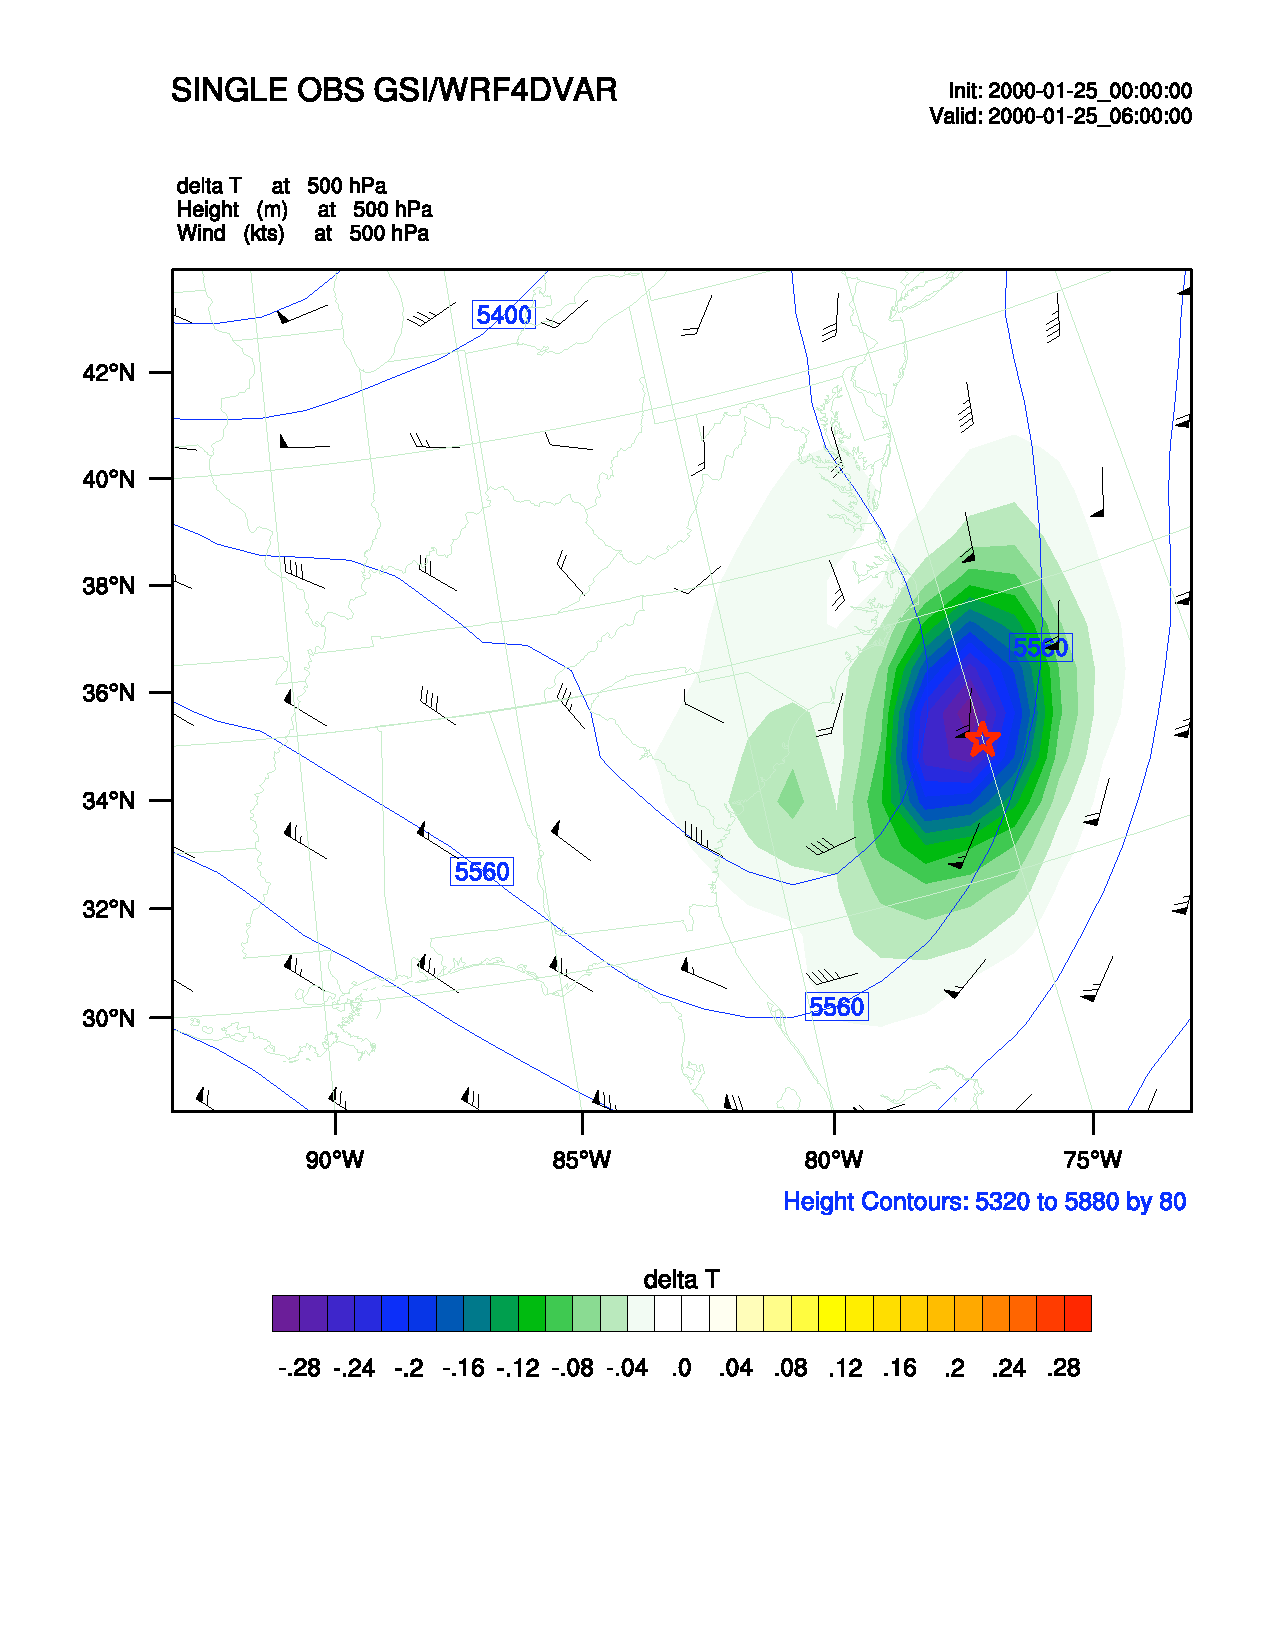
\includegraphics[scale=0.25, trim=10 5 10 10, clip]{gsi4dvar.pdf} & 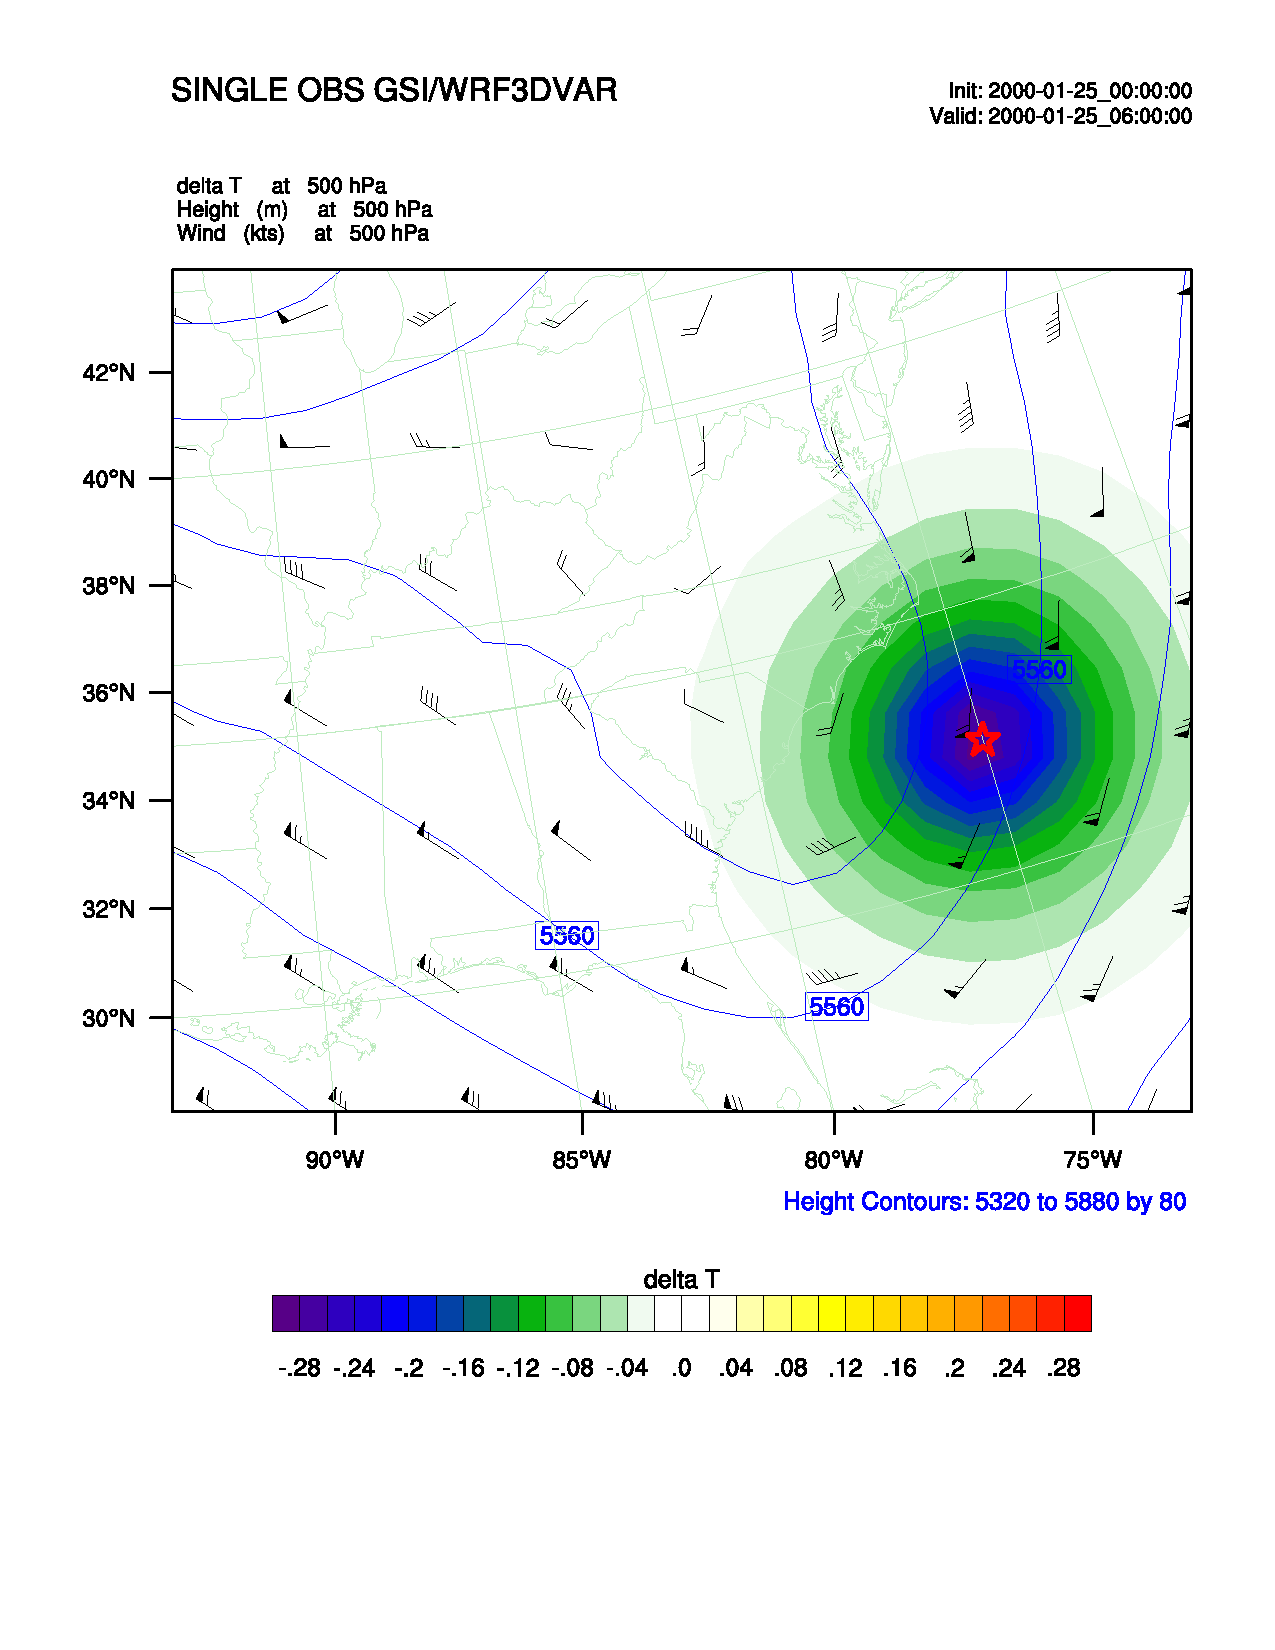
\includegraphics[scale=0.25, trim=10 5 10 10, clip]{gsi3dvar.pdf}
\end{tabular}
}

\fst{Single observation exp. II}{
\begin{itemize}
	\item Initial time: $2000\_01\_25\_00:00:00$
	\item Ending time: $2000\_01\_25\_06:00:00$
	\item Observation: 500 mb Temperature at {\color{red}ending time} \\
	          $O-B=-1.04K$
	\item To investigate the impact of an observation close to boundary.
\end{itemize}
}

\frame{
\begin{columns}[c]
\column{6cm}
\includemovie[
  poster=boundary.pdf,
  text={}
]{6.0cm}{7.5cm}{gsiwrf4dvar_boundary.mpeg}
\column[c]{3.5cm}
\begin{block}{Remarks}
\tiny{Forecasted 500mb T difference \\(DA forecast - reference forecast)}
\begin{itemize}
	\item {\color{red}$\star$} is the location of obs. at the ending time (6h).
	\item \tiny{Initial perturbation is on the upstream of the obs.}
	\item \tiny{Evolved perturbation at 6h miss the obs. location}
	\item \tiny{Without LBC control, it is hard to fit the obs.}
\end{itemize}
\end{block}
\end{columns}
}

\subsection{Tutorial case}

\begin{frame}[fragile]
\frametitle{Tutorial case -- Observation Usage}
\begin{center}
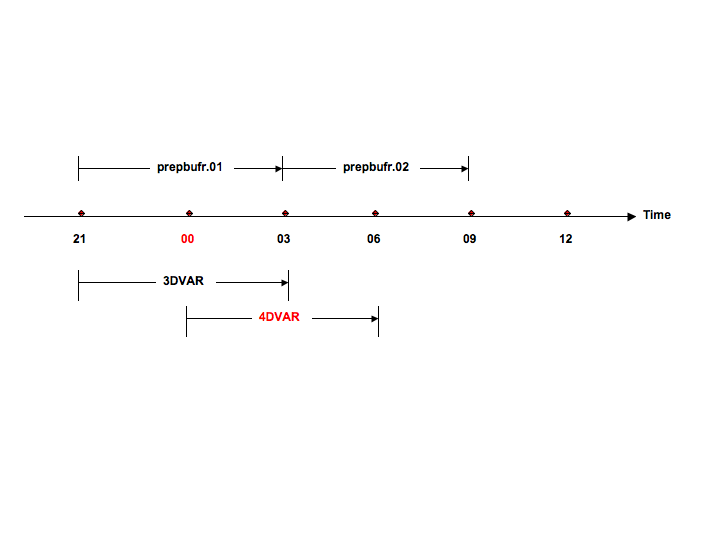
\includegraphics[scale=0.40, trim=25 200 50 150, clip]{obs_usage} 
\end{center}\pause
\begin{columns}[c]
\column{5cm}
\setbeamercolor{postit}{fg=black, bg=yellow}
\begin{beamerboxesrounded}[ lower=postit,shadow=true]{3DVAR}
{\tiny
\begin{verbatim}
   0:OBS_PARA: ps                       13842
   0:OBS_PARA: t                        20114
   0:OBS_PARA: q                        18743
   0:OBS_PARA: uv                       30894
   0:OBS_PARA: spd                         48
   0:OBS_PARA: sst                        503
   0:OBS_PARA: pw                         880
   ----------------Total--------------------
   47675
\end{verbatim}
}
\end{beamerboxesrounded}
\column{5cm}
\setbeamercolor{postit}{fg=black, bg=yellow}
\begin{beamerboxesrounded}[ lower=postit,shadow=true]{4DVAR}
{\tiny
\begin{verbatim}
   0:OBS_PARA: ps                       13585
   0:OBS_PARA: t                        20639
   0:OBS_PARA: q                        19180
   0:OBS_PARA: uv                       28802
   0:OBS_PARA: spd                         80
   0:OBS_PARA: sst                        494
   0:OBS_PARA: pw                         766
   ------------------------------
   0:OBS_PARA: ps                          10
   0:OBS_PARA: t                          552
   0:OBS_PARA: q                          490
   0:OBS_PARA: uv                         568
   ----------------Total-------------------
   45040
\end{verbatim}
}
\end{beamerboxesrounded}
\end{columns}
\end{frame}


\frame{
\frametitle{Cost functions and gradients --scaled by ALOG10}
\begin{tabular}{l r}
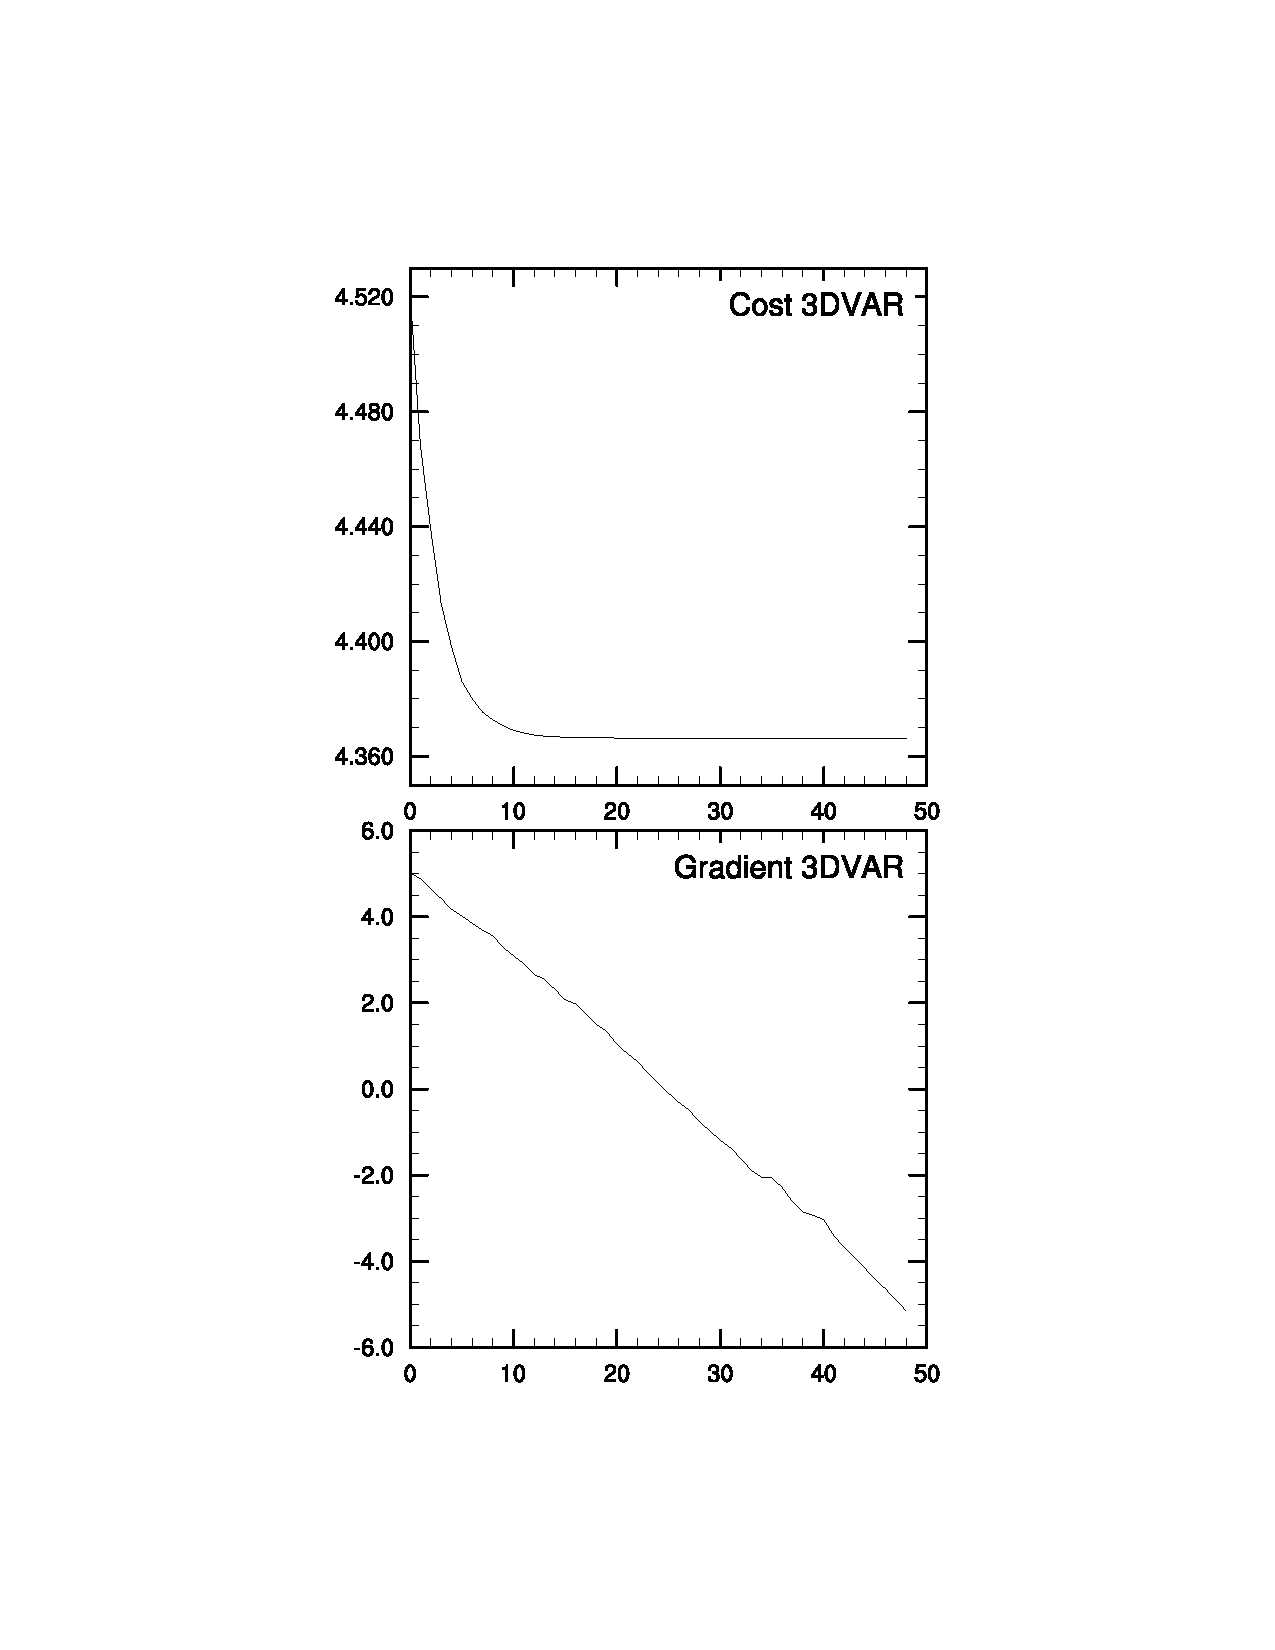
\includegraphics[scale=0.30, trim=10 5 100 50, clip]{3dvar_cost_grad.pdf} & 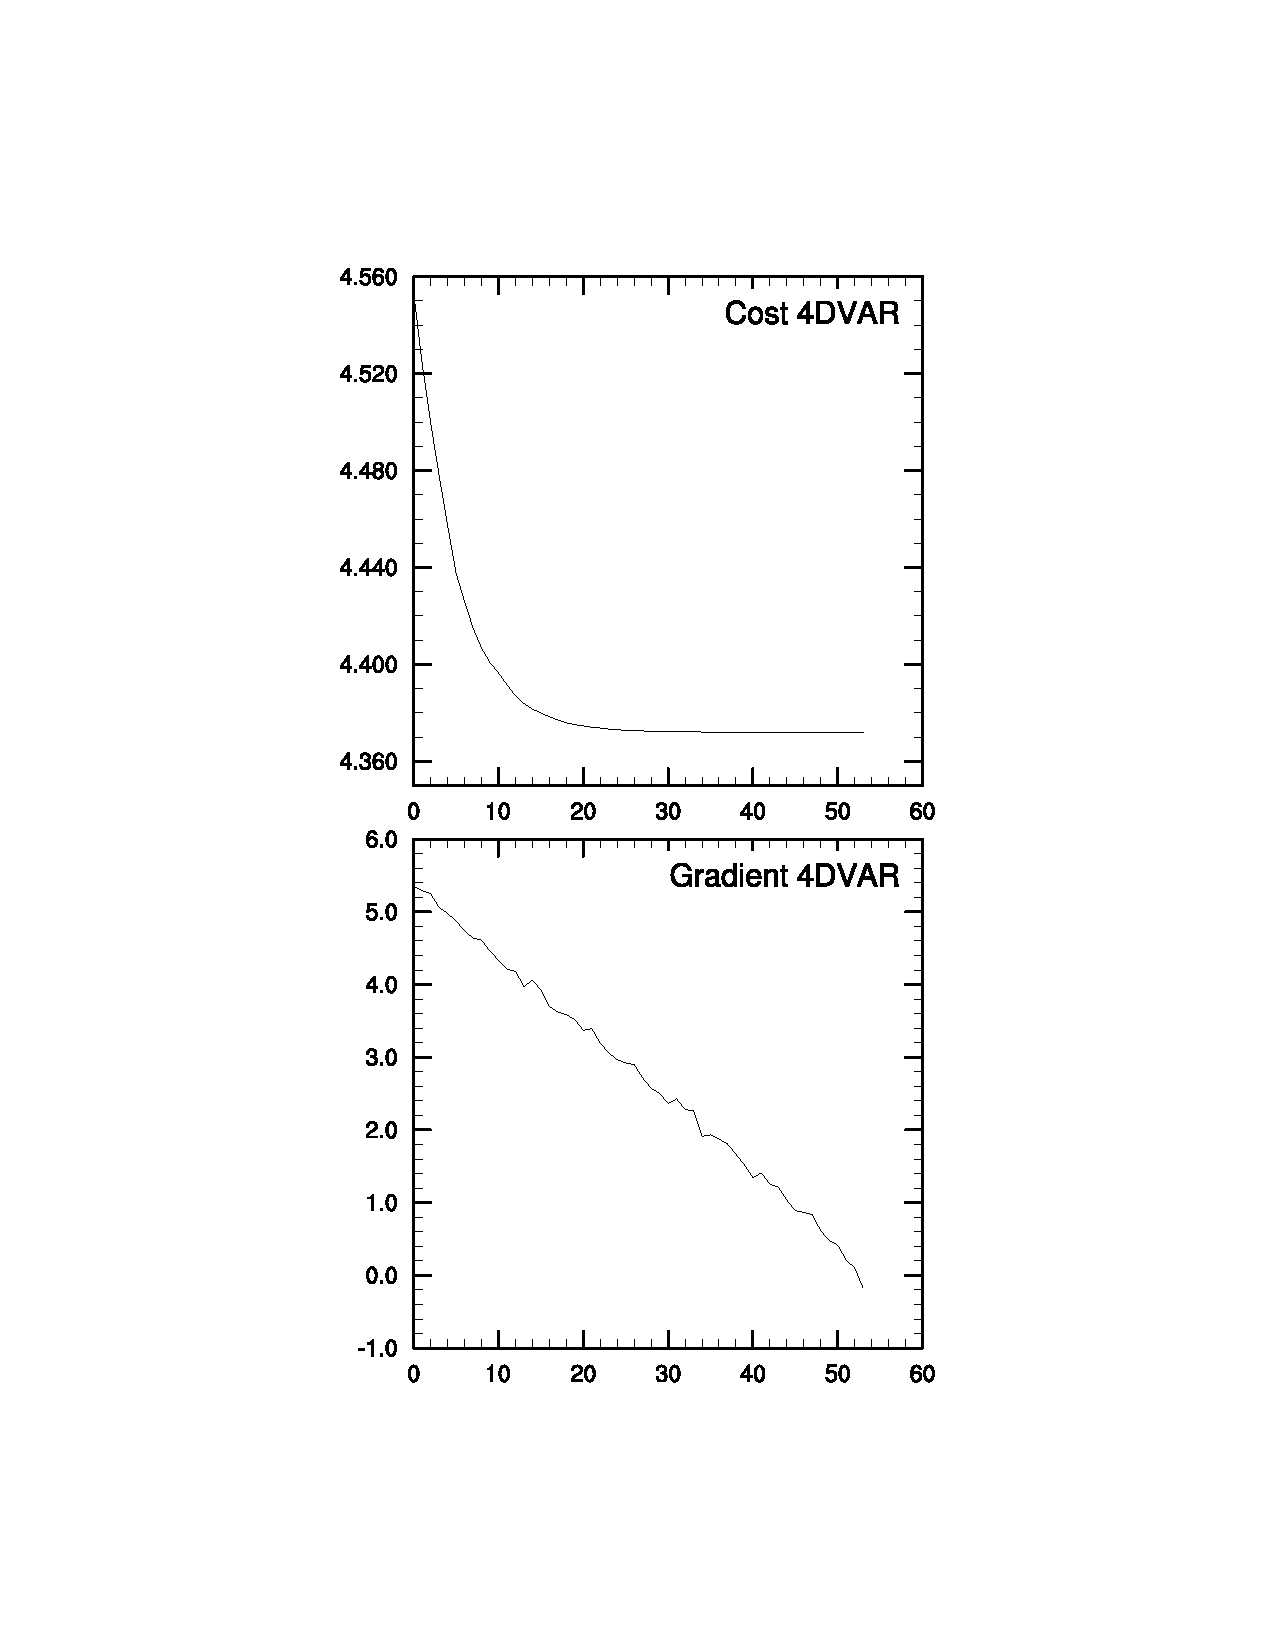
\includegraphics[scale=0.30, trim=150 5 10 50, clip]{4dvar_cost_grad.pdf}
\end{tabular}
}

\frame{
\frametitle{Sample increments comparison -- U, T}
\begin{tabular}{l r}
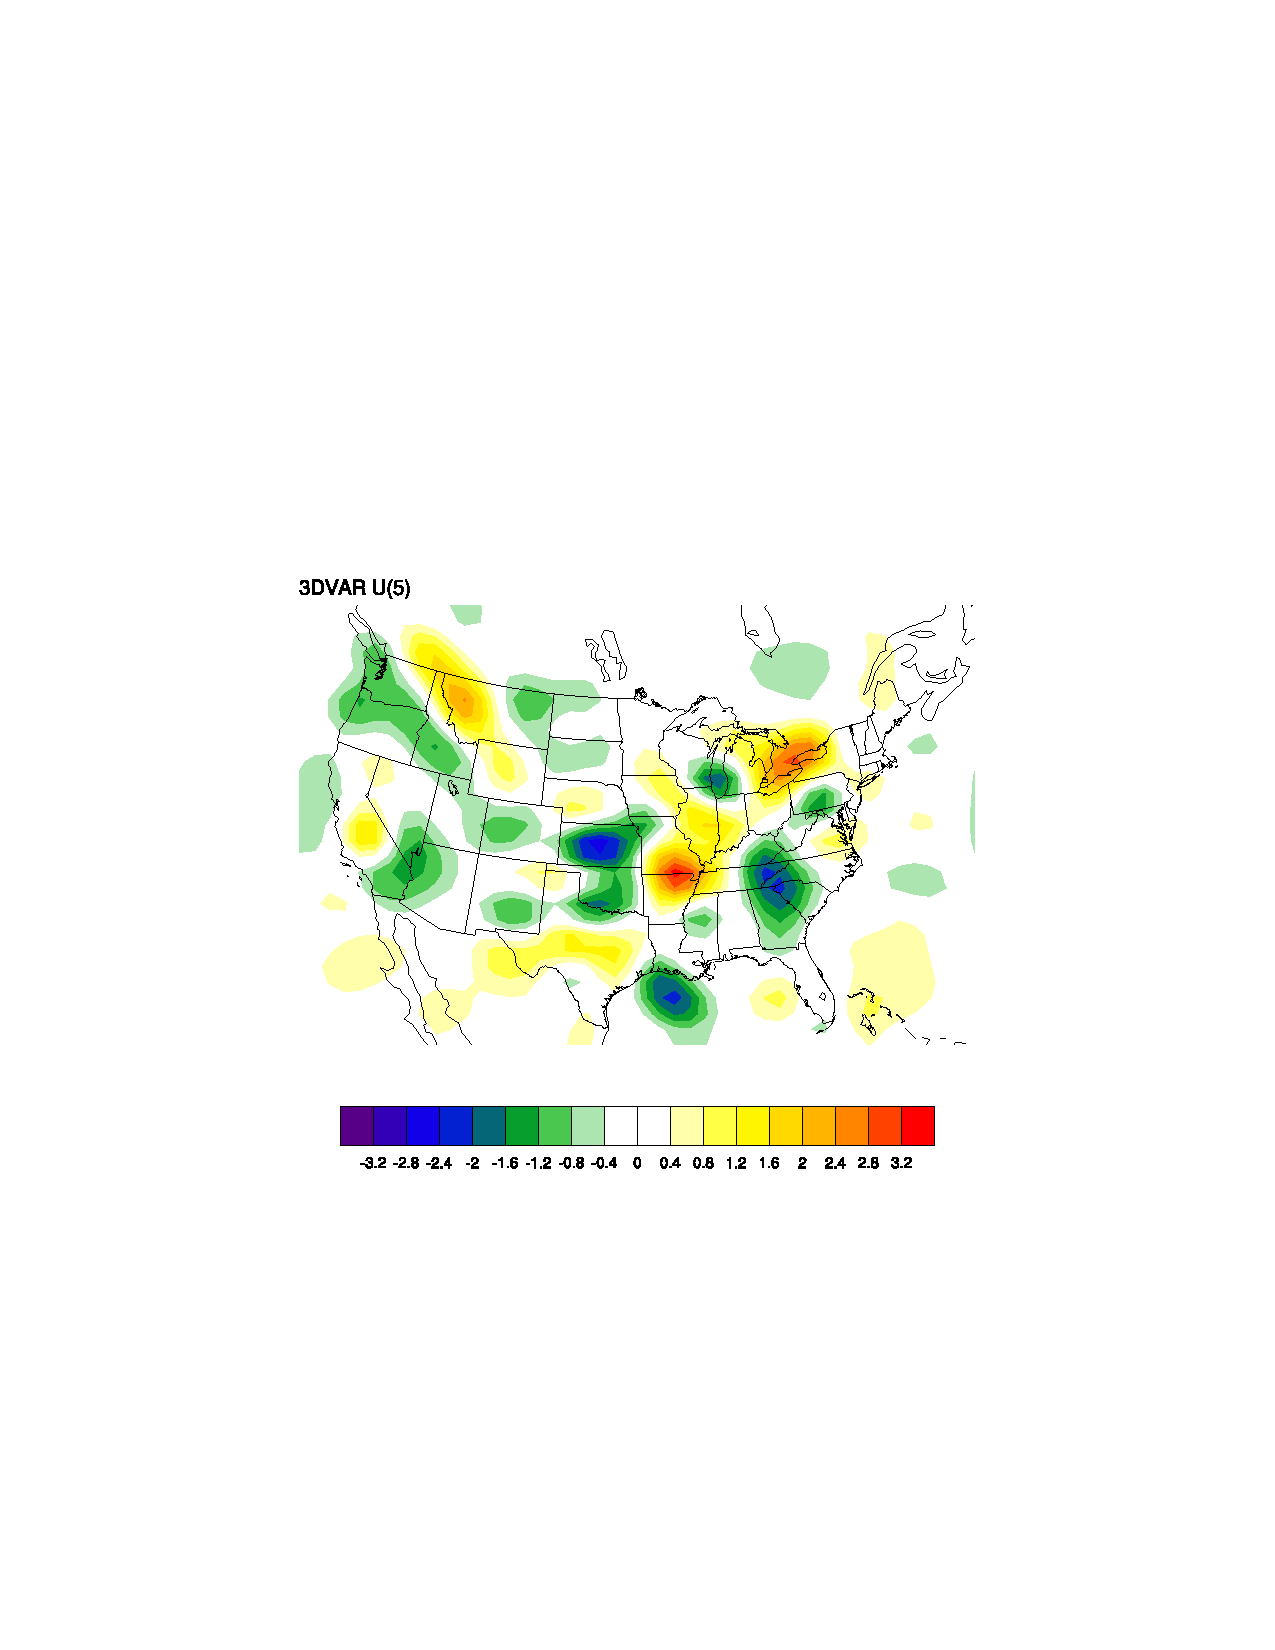
\includegraphics[scale=0.30, trim=50 230 100 250, clip]{3dvar_u_5_inc} & 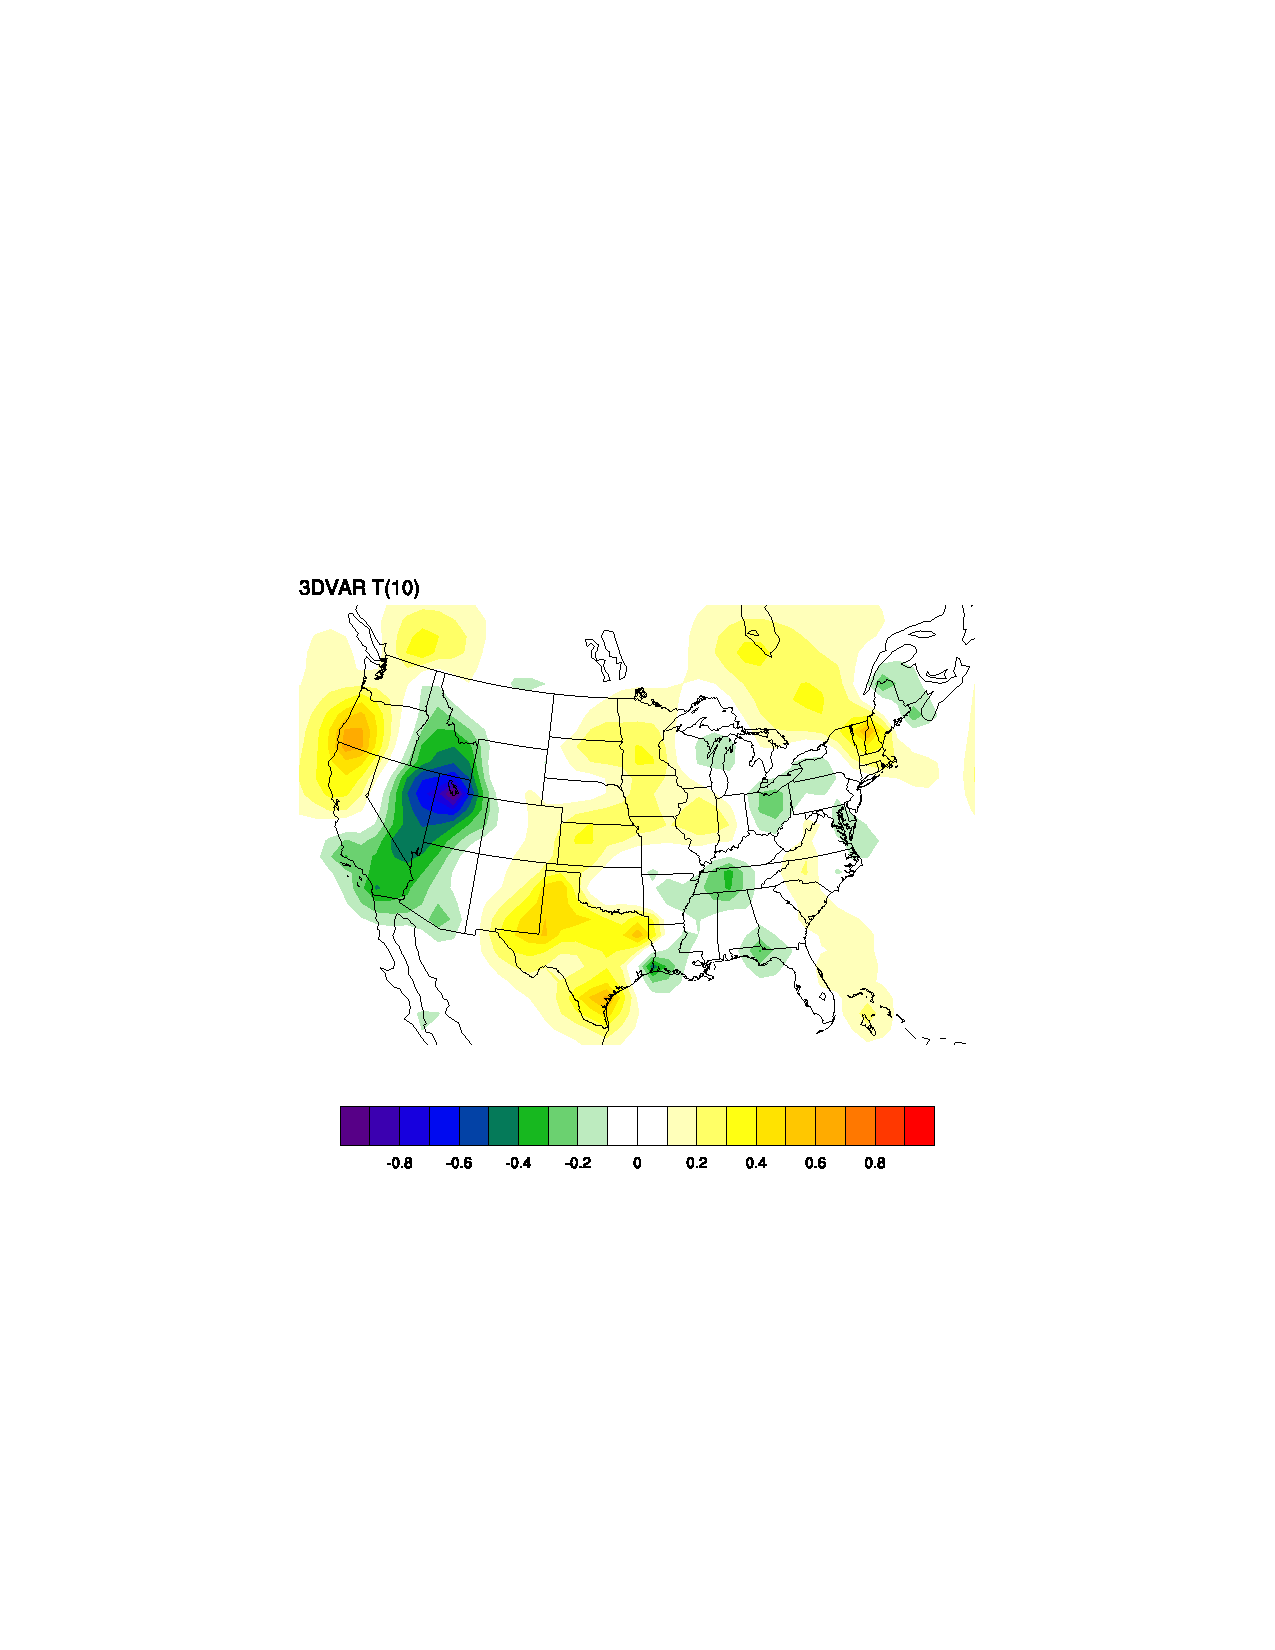
\includegraphics[scale=0.30, trim=100 230 100 250, clip]{3dvar_t_10_inc} \\
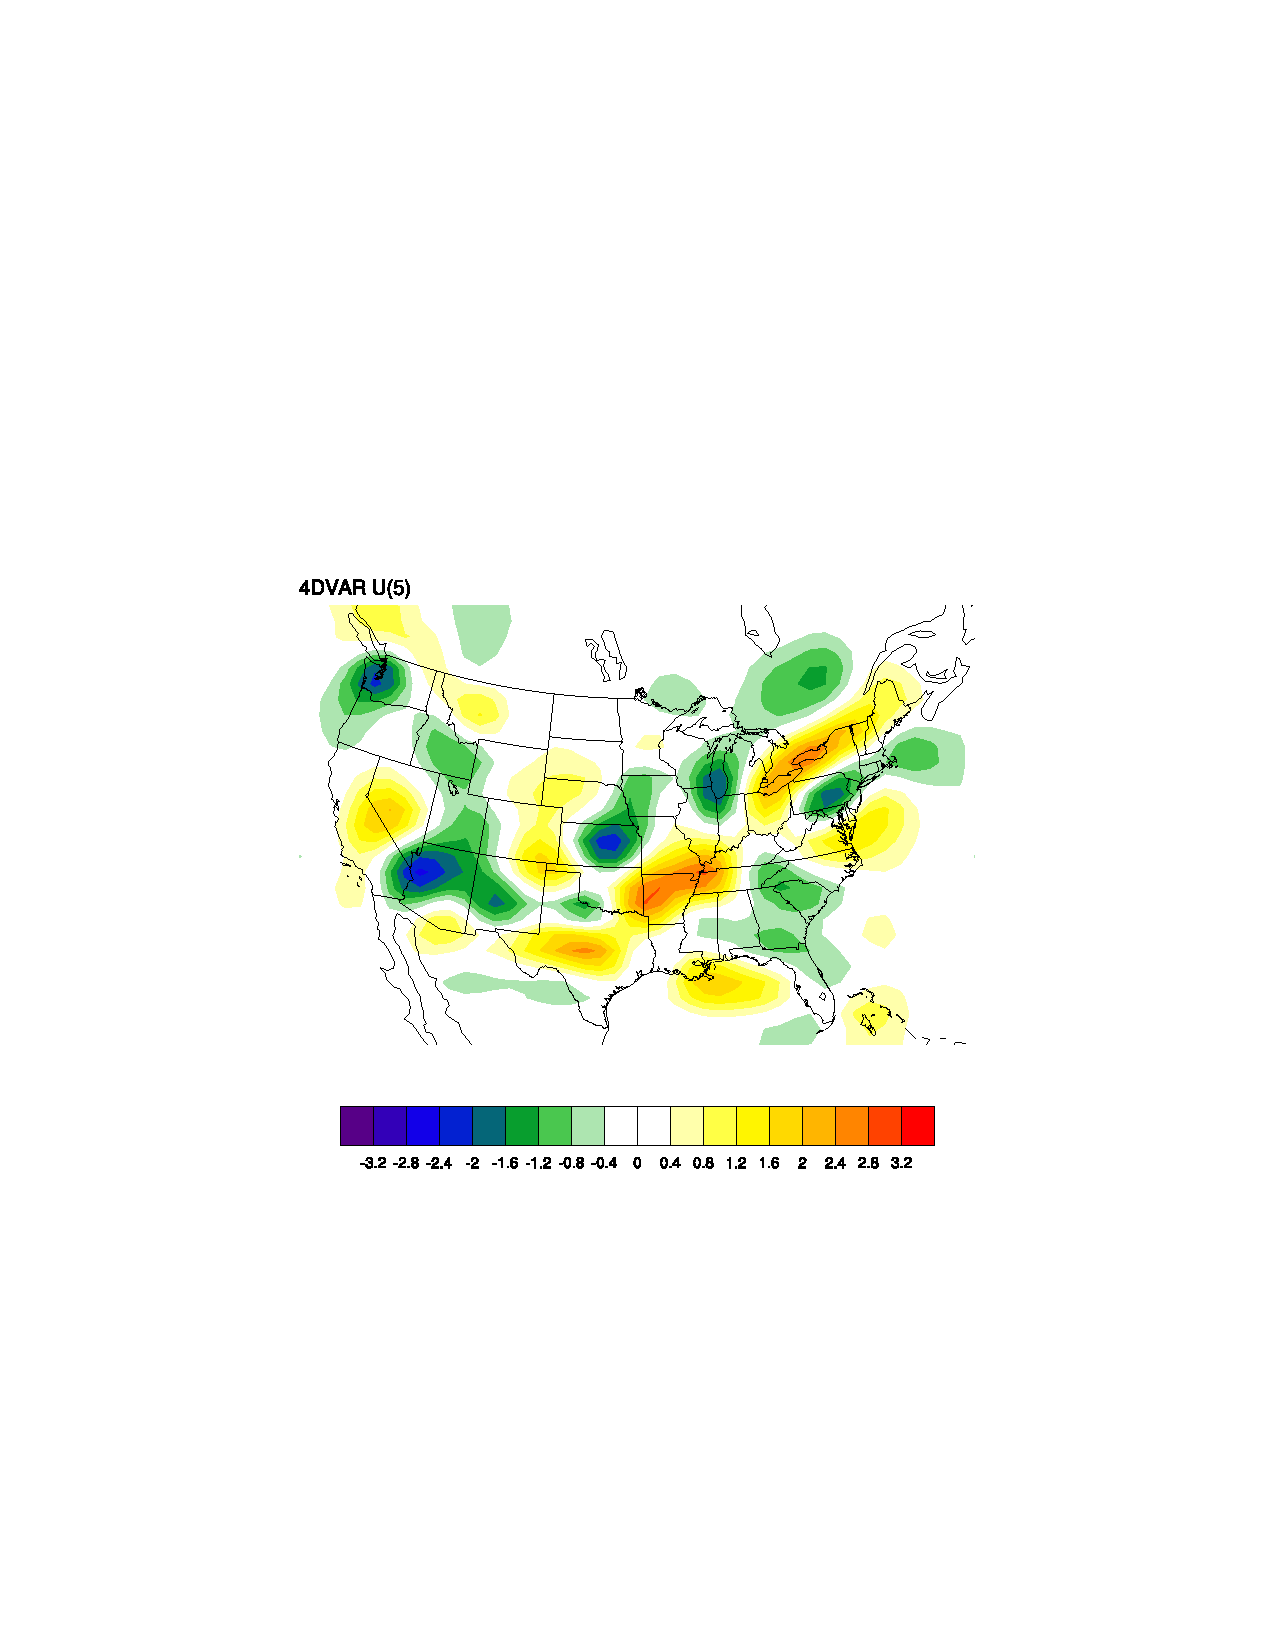
\includegraphics[scale=0.30, trim=50 160 100 250, clip]{4dvar_u_5_inc} & 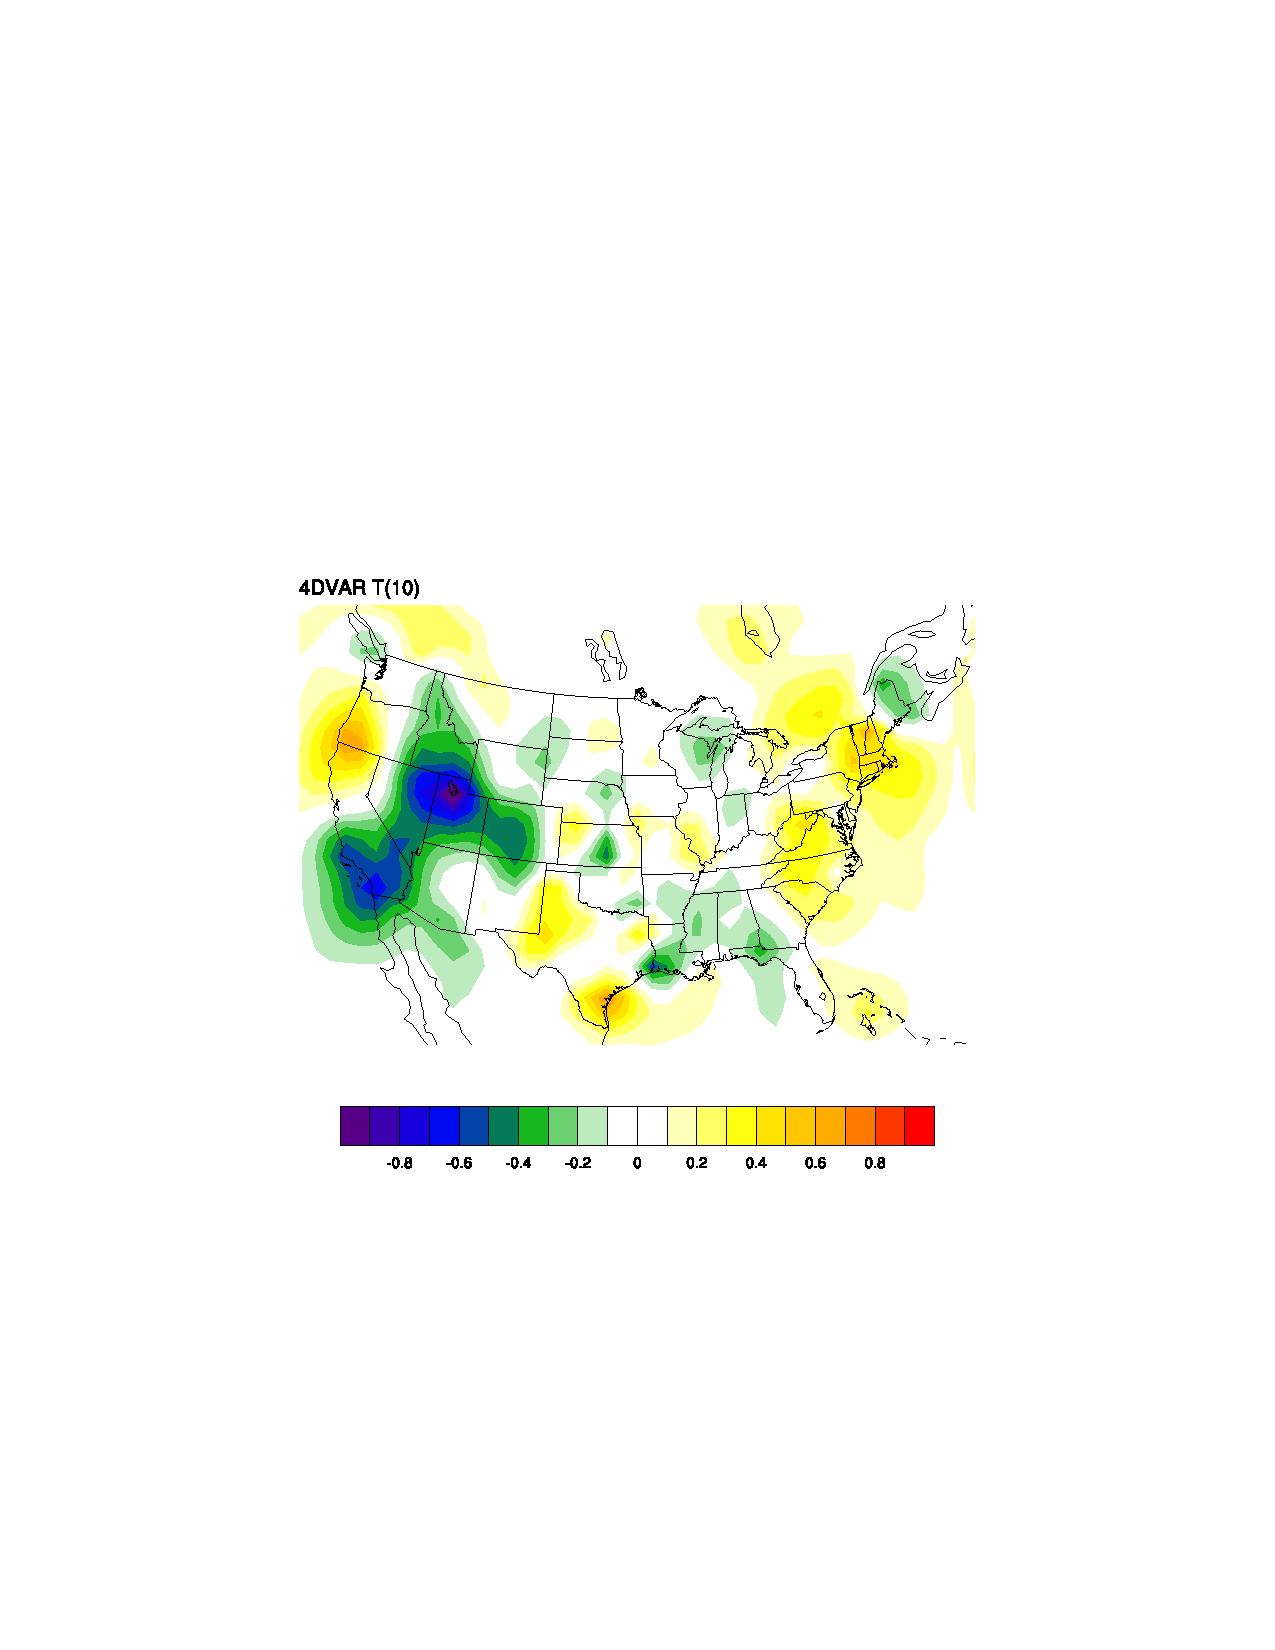
\includegraphics[scale=0.30, trim=100 160 100 250, clip]{4dvar_t_10_inc}
\end{tabular}
}

\frame{
\frametitle{Sample increments comparison -- MU, QVAPOR}
\begin{tabular}{l r}
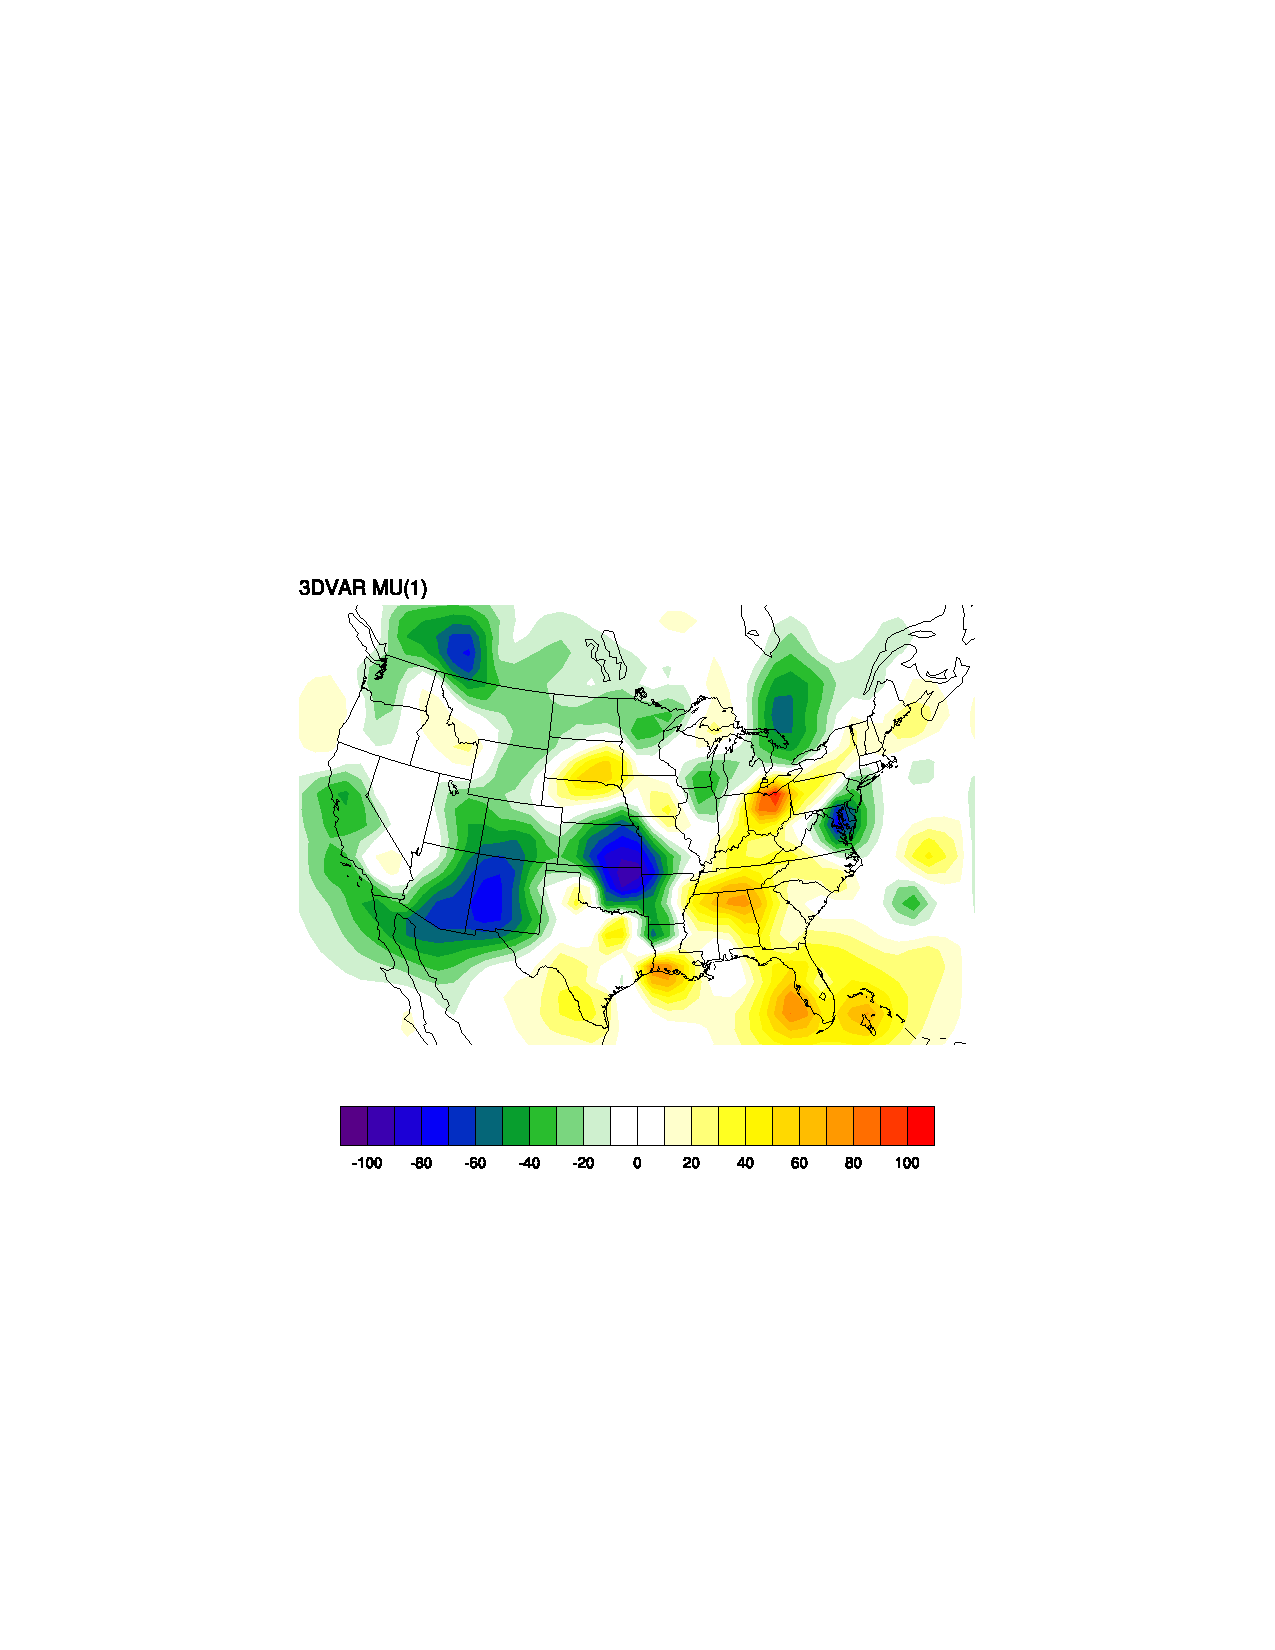
\includegraphics[scale=0.30, trim=50 230 100 250, clip]{3dvar_mu_inc} & 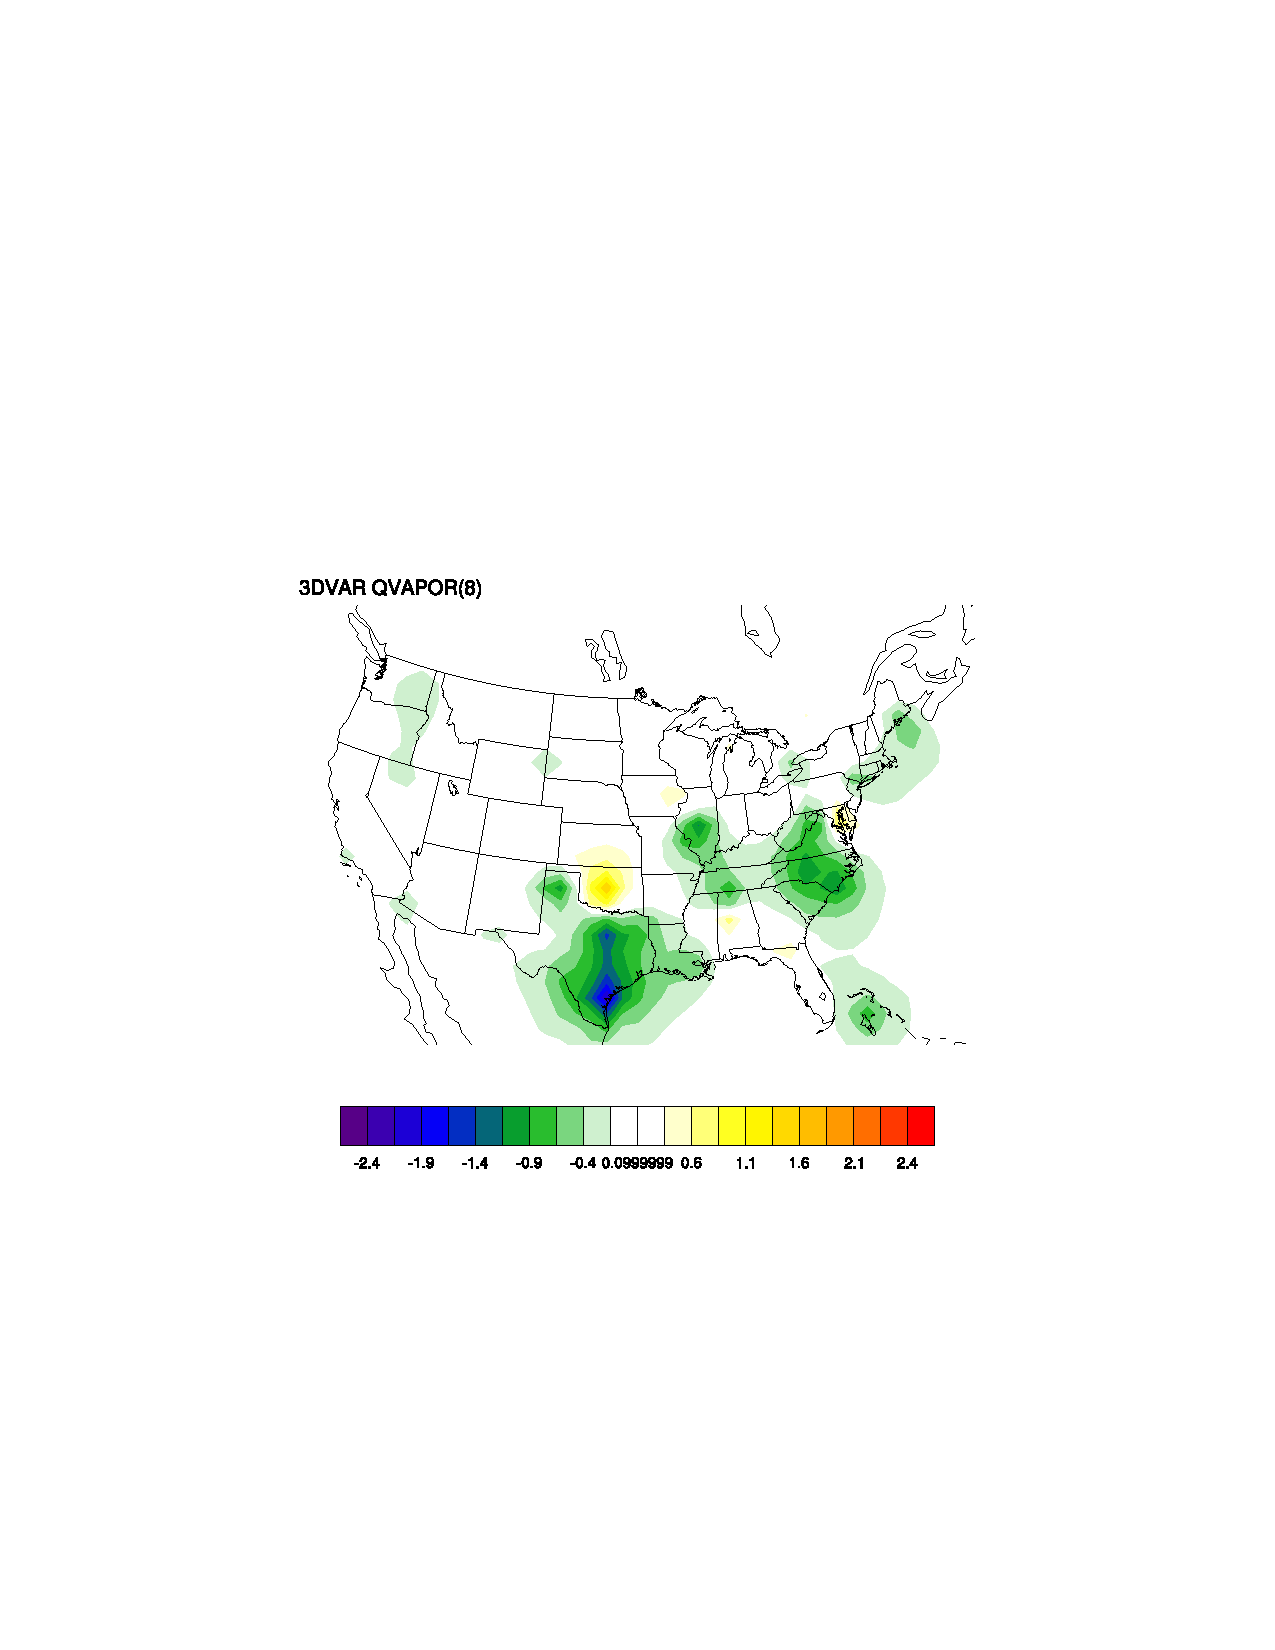
\includegraphics[scale=0.30, trim=100 230 100 250, clip]{3dvar_q_8_inc} \\
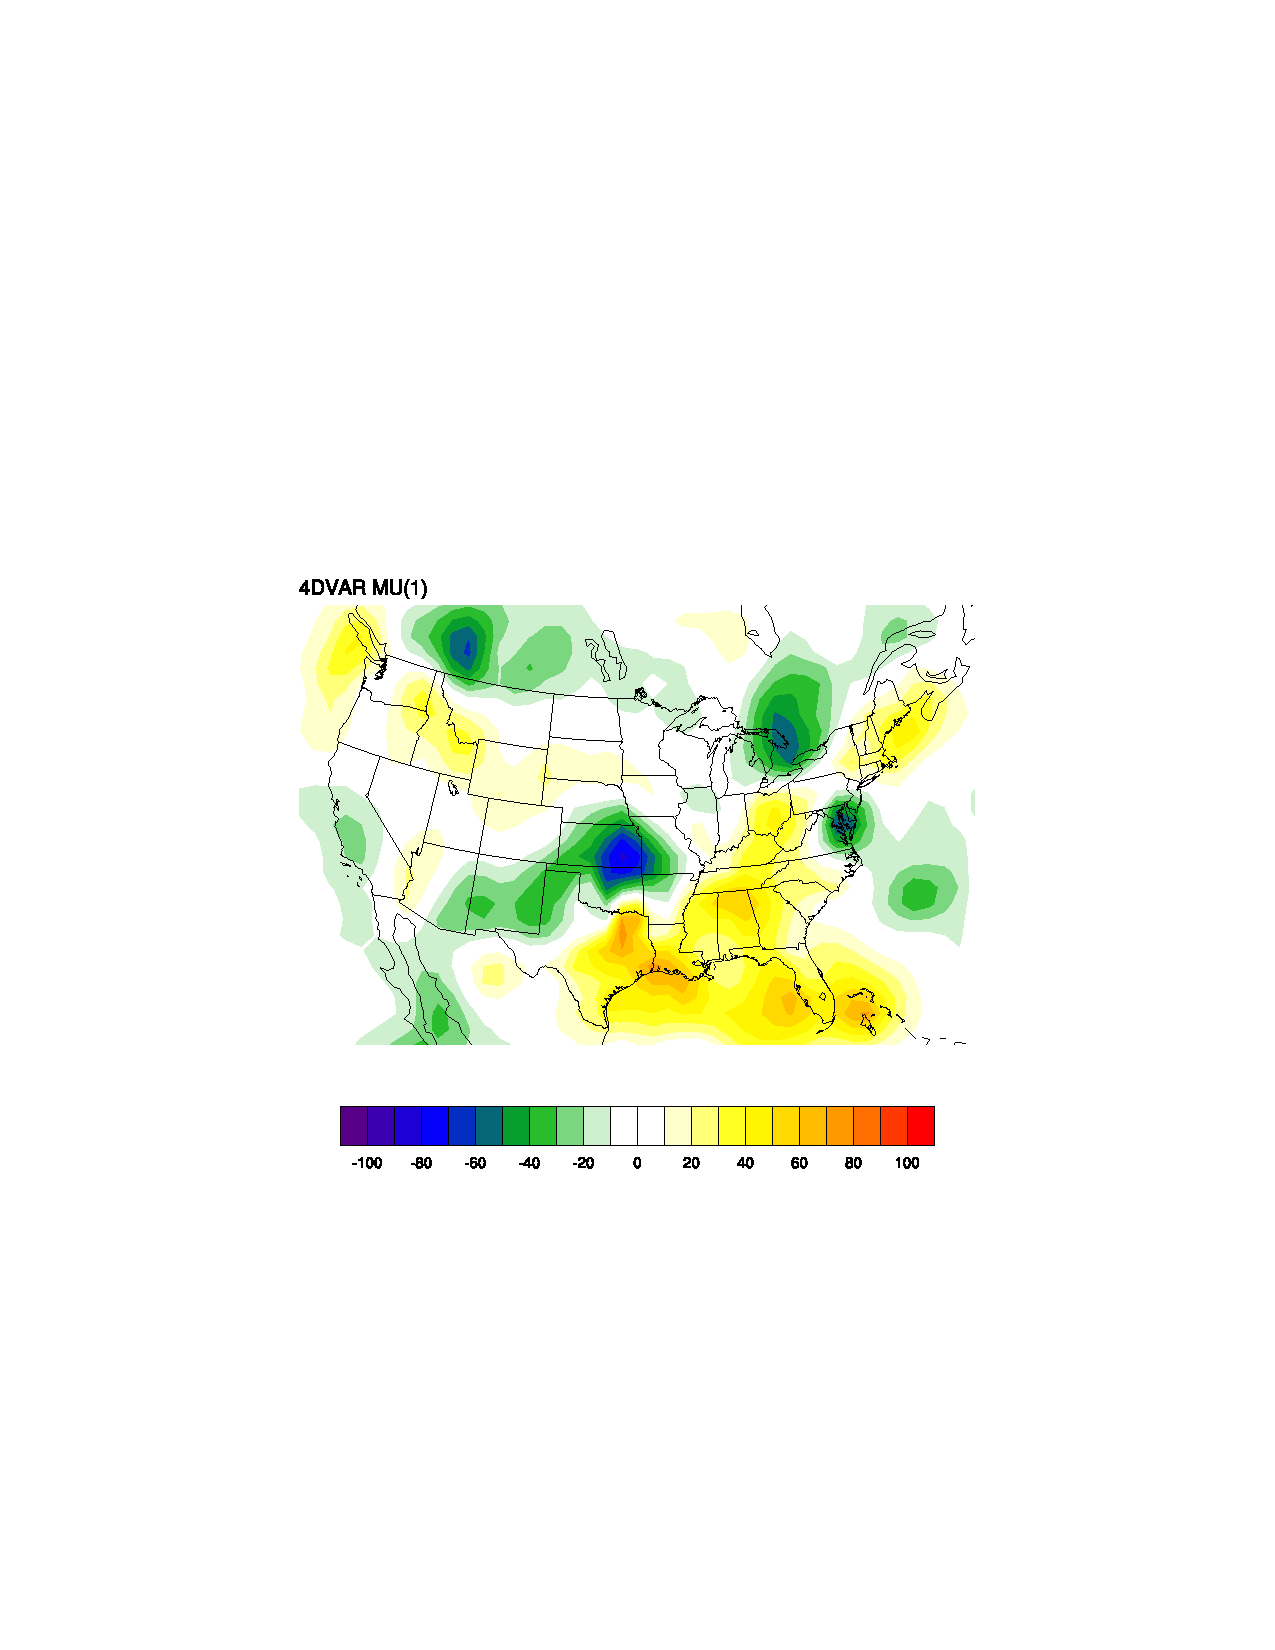
\includegraphics[scale=0.30, trim=50 160 100 250, clip]{4dvar_mu_inc} & 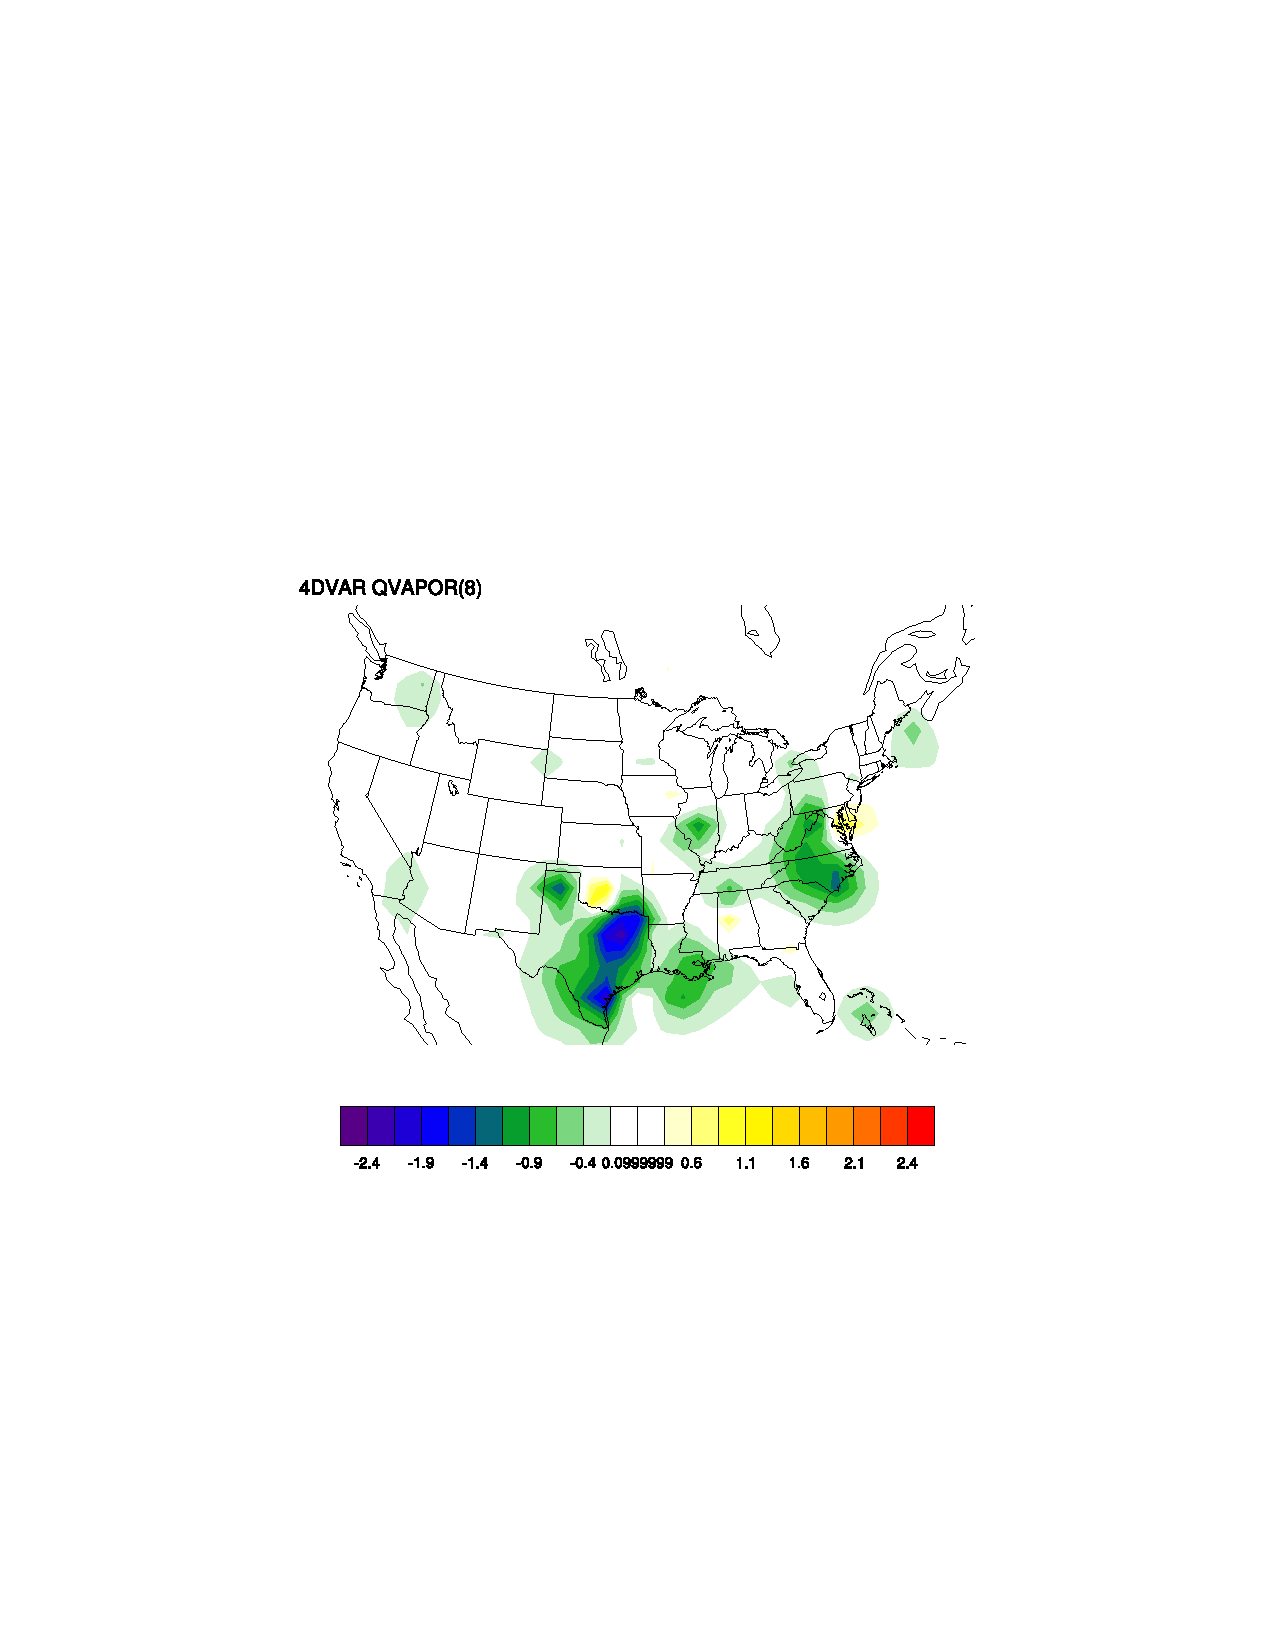
\includegraphics[scale=0.30, trim=100 160 100 250, clip]{4dvar_q_8_inc}
\end{tabular}
}

\subsection{Real case}

\frame{
\frametitle{Experiment configuration}
\begin{itemize}
	\item Grids: 105x72x28L
	\item Resolution: 60km
	\item Period: 2007091100-2007092600 @0Z,6Z,12Z,18Z
	\item First guess is the 12h forecast from NCEP FNL
	\item 48h forecast from FG, 3DVAR and 4DVAR
	\item Verified against NCAR archived little\_r format data, filtered by FNL.
\end{itemize}
\begin{center}
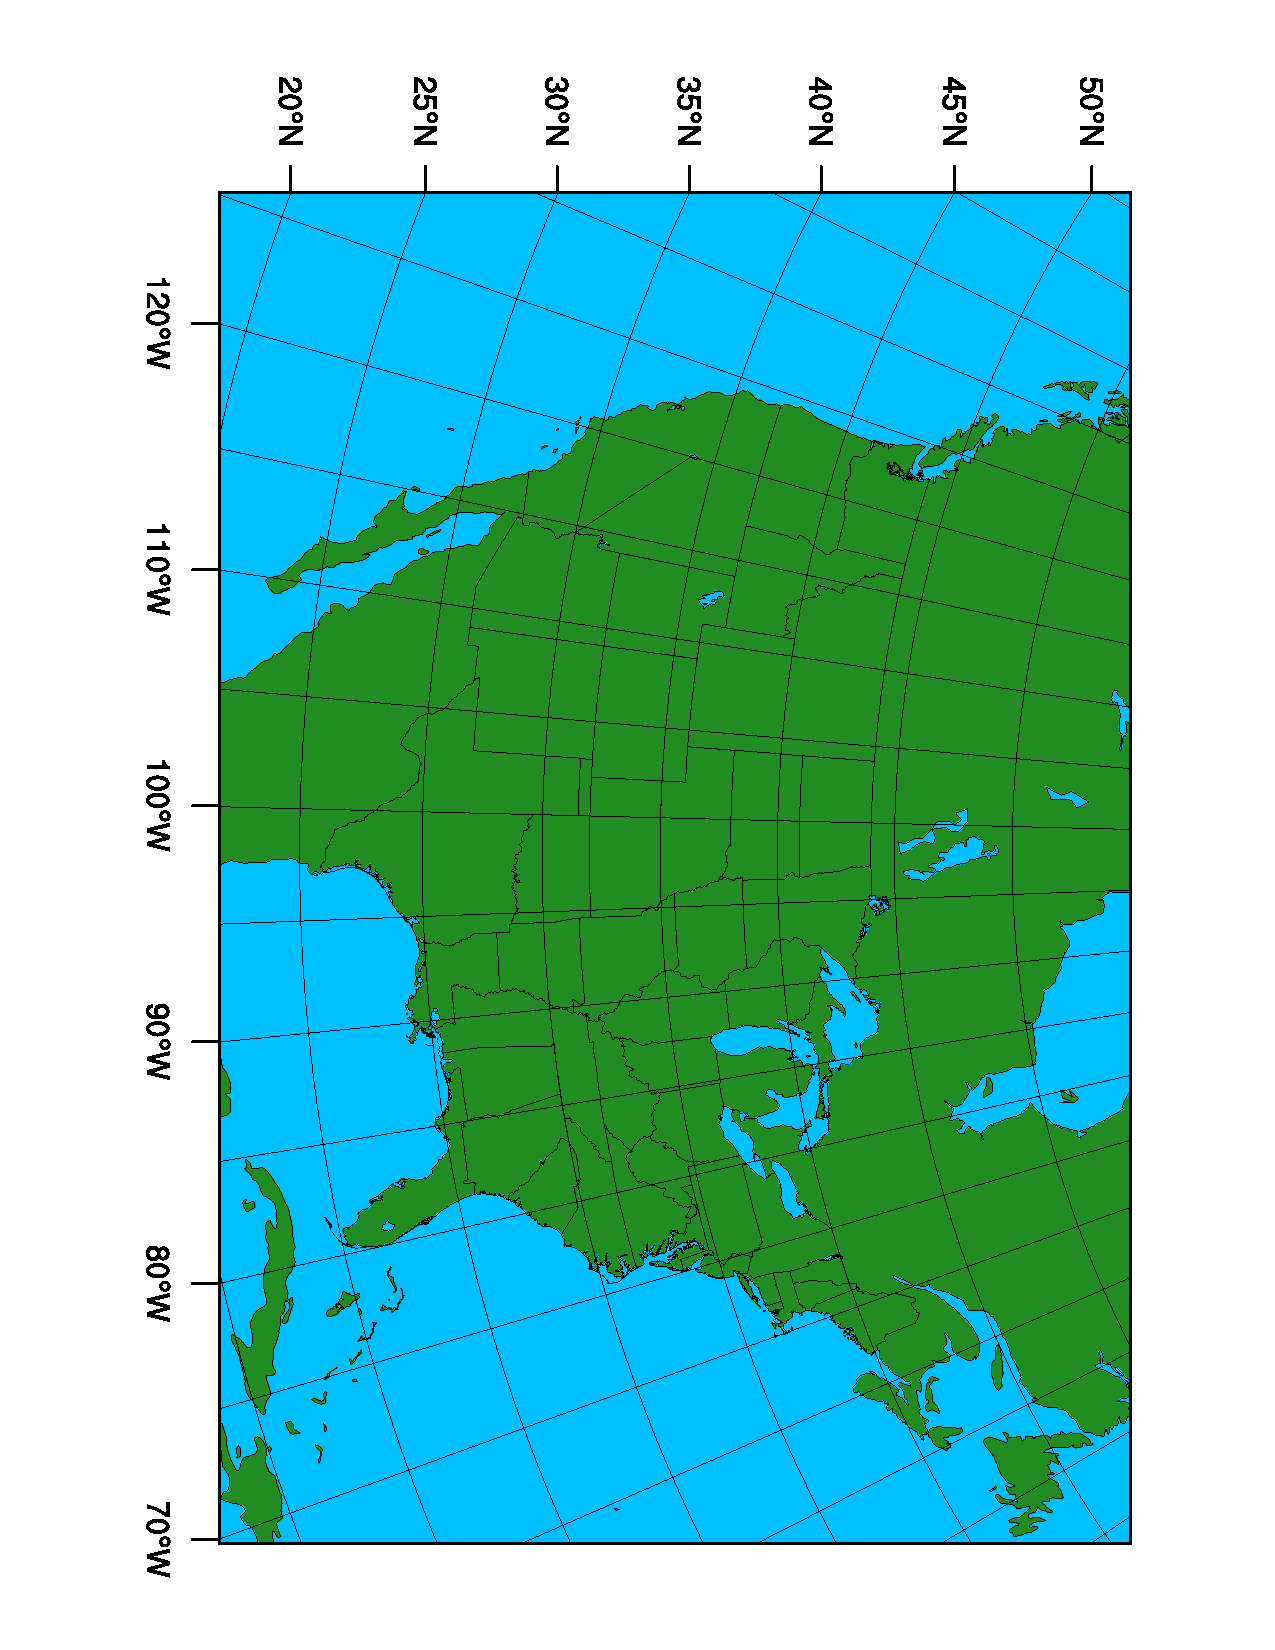
\includegraphics[scale=0.25, trim=0 0 50 0, clip, angle=90]{domain.pdf} 
\end{center}
}

\frame{
\frametitle{RMSE Verification---00h}
\begin{center}
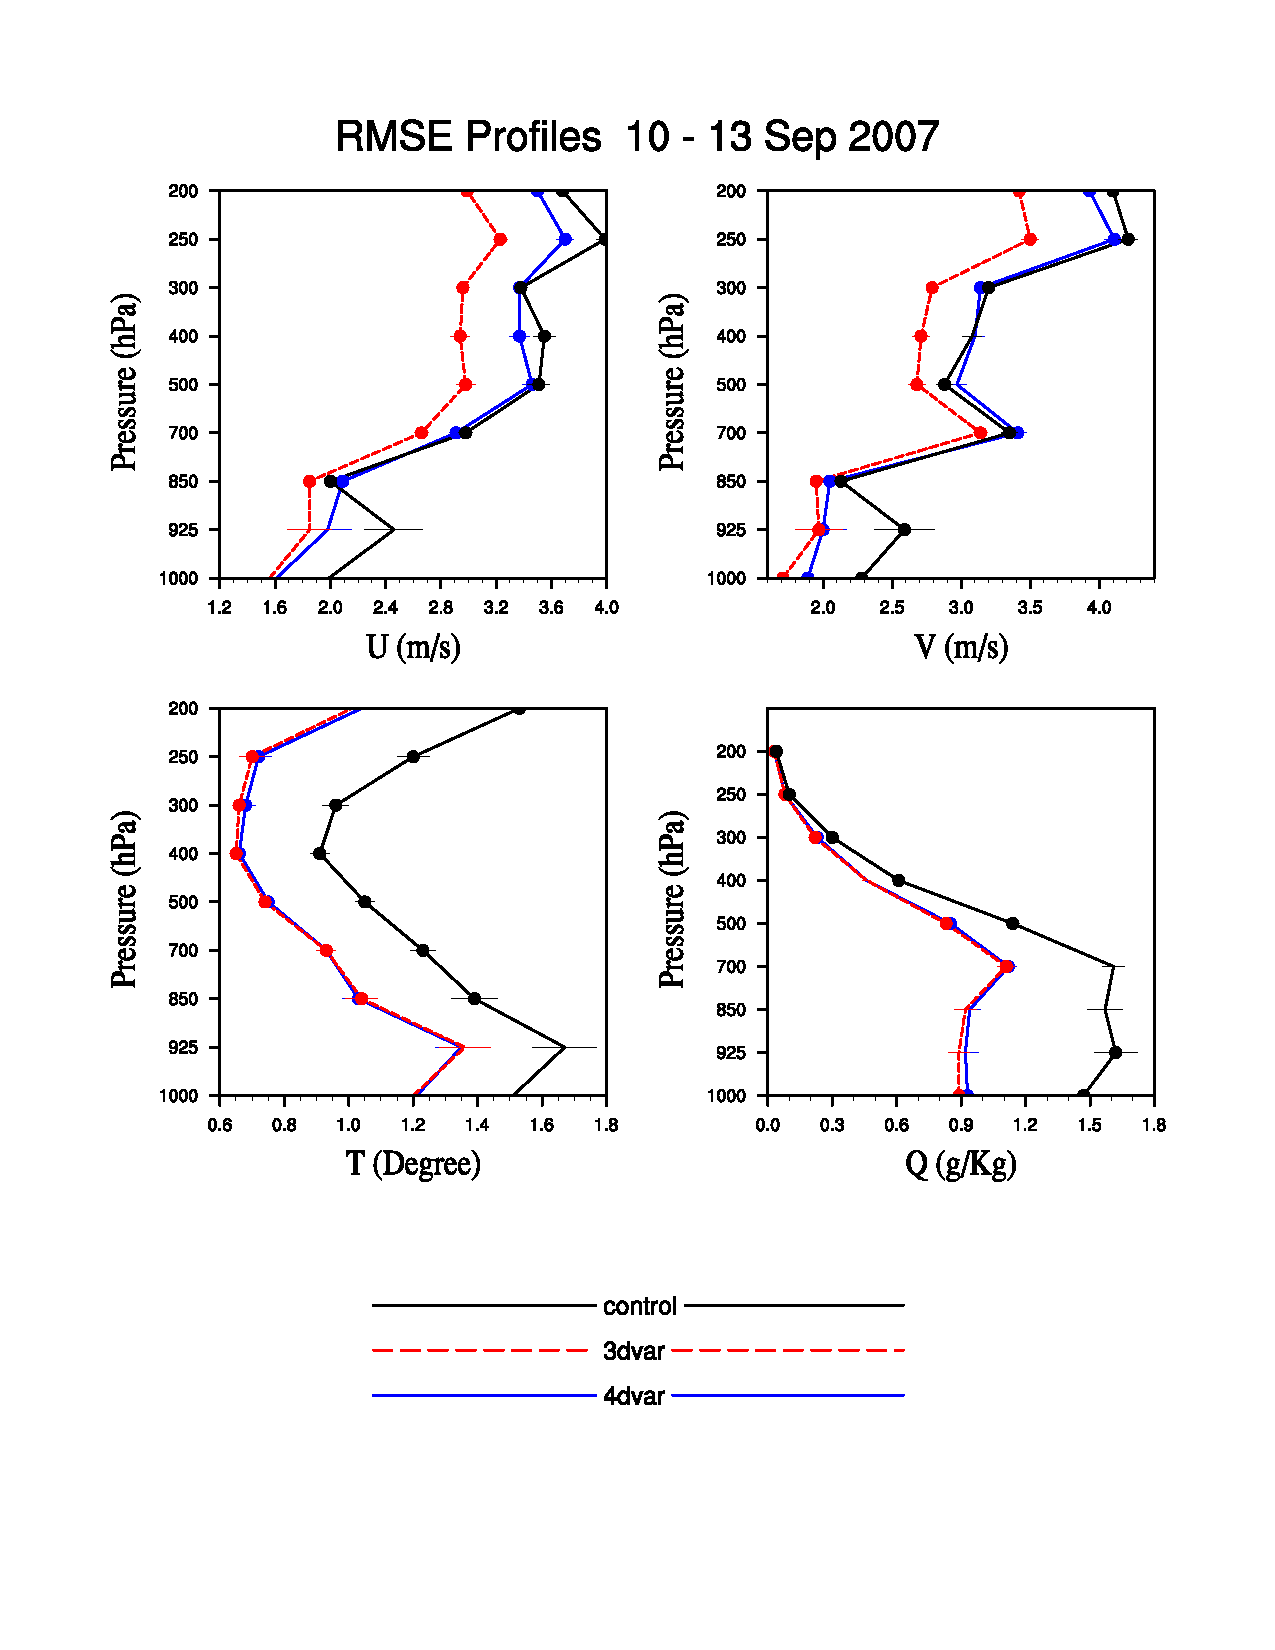
\includegraphics[scale=0.33, trim=0 0 0 80, clip]{Profile_RMSE_0.pdf}
\end{center}
}

\frame{
\frametitle{RMSE Verification---06h}
\begin{center}
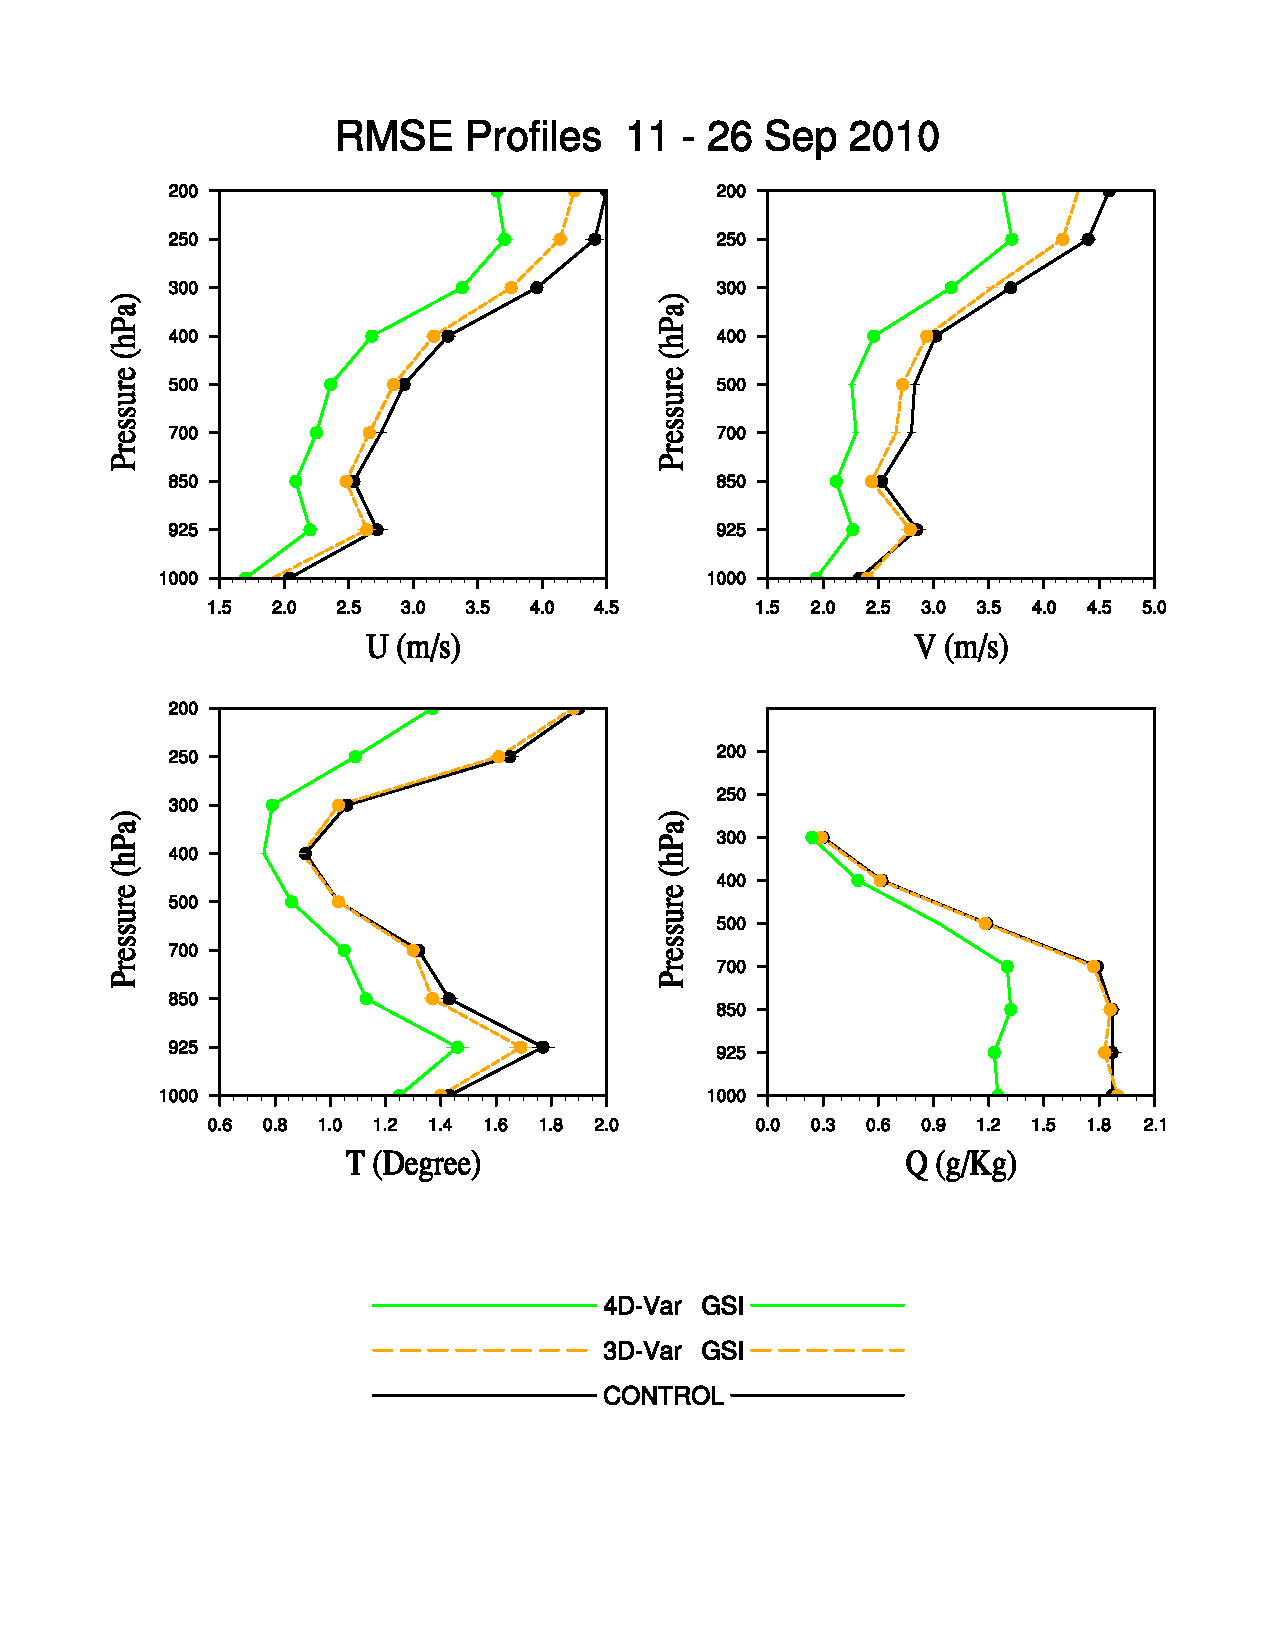
\includegraphics[scale=0.33, trim=0 0 0 80, clip]{Profile_RMSE_6.pdf}
\end{center}
}

\frame{
\frametitle{RMSE Verification---12h}
\begin{center}
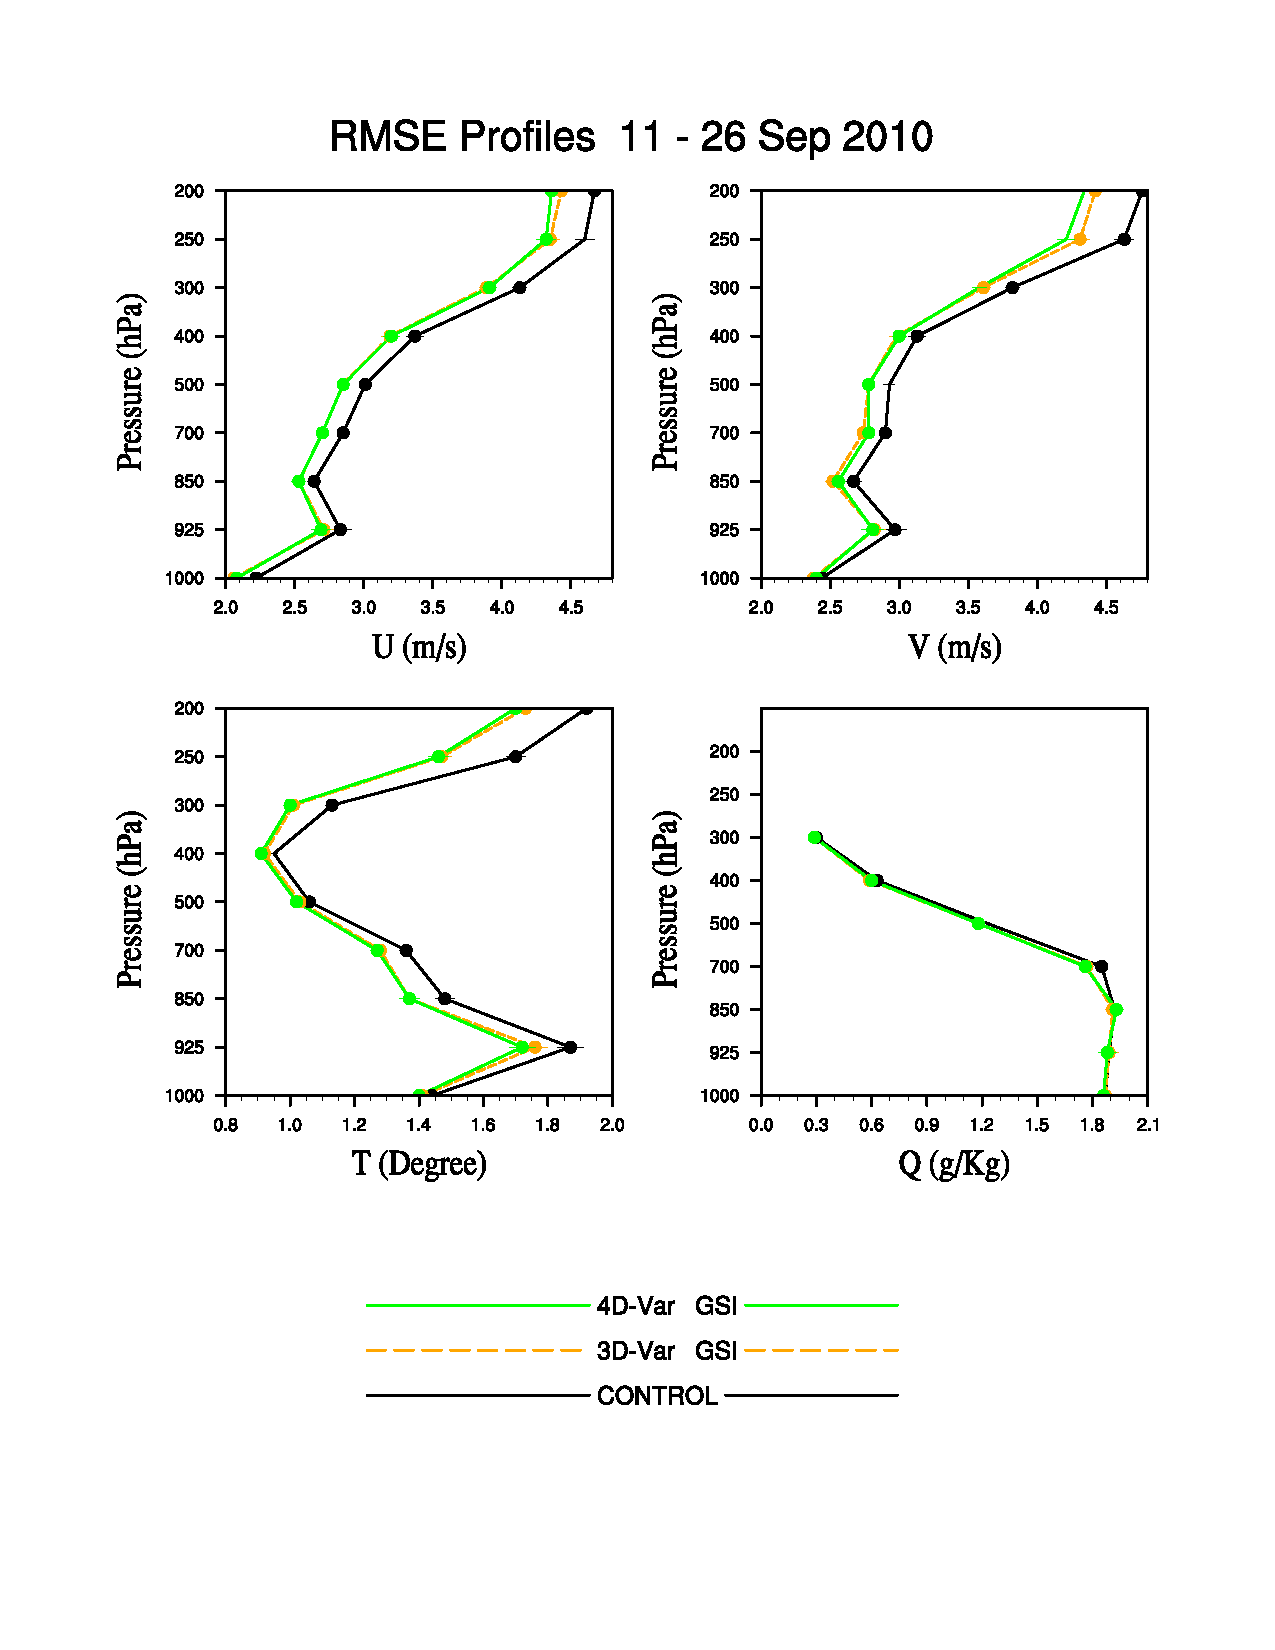
\includegraphics[scale=0.33, trim=0 0 0 80, clip]{Profile_RMSE_12.pdf}
\end{center}
}

\frame{
\frametitle{RMSE Verification---18h}
\begin{center}
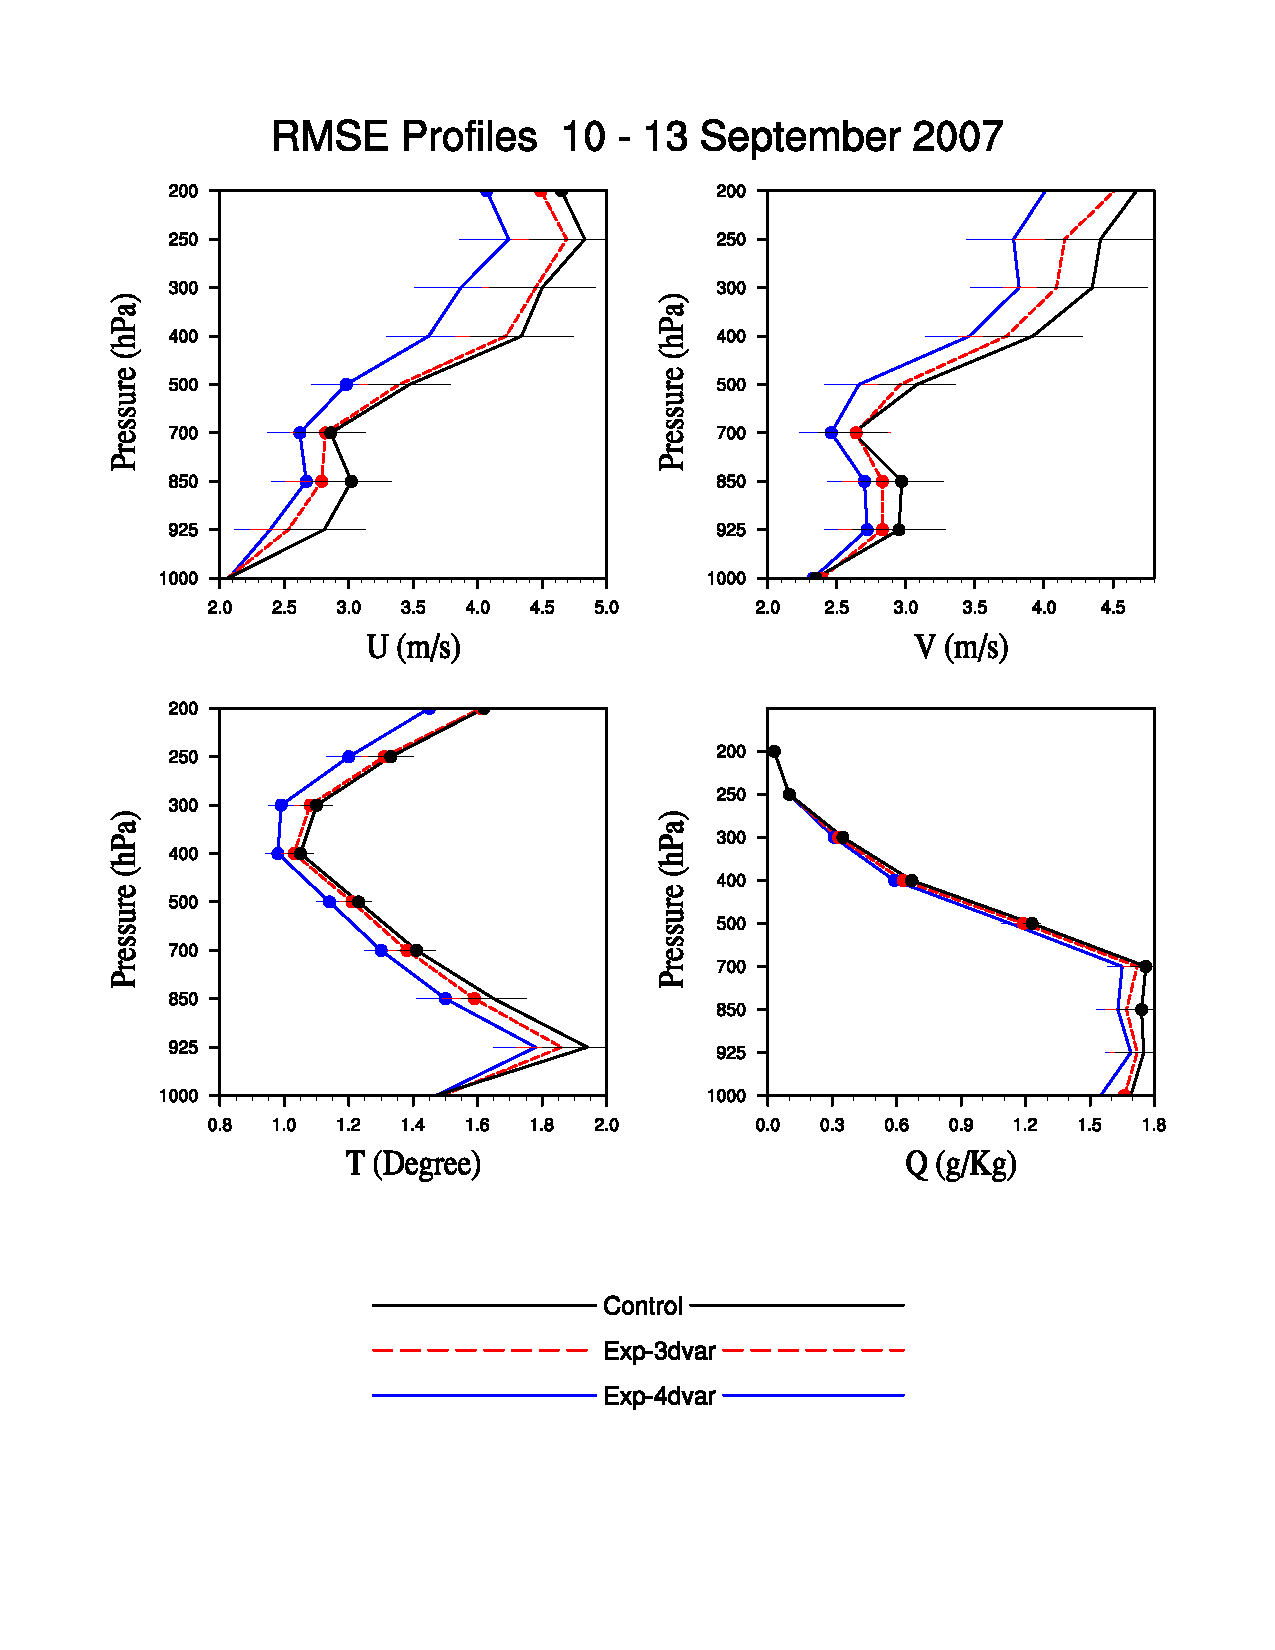
\includegraphics[scale=0.33, trim=0 0 0 80, clip]{Profile_RMSE_18.pdf}
\end{center}
}

\frame{
\frametitle{RMSE Verification---24h}
\begin{center}
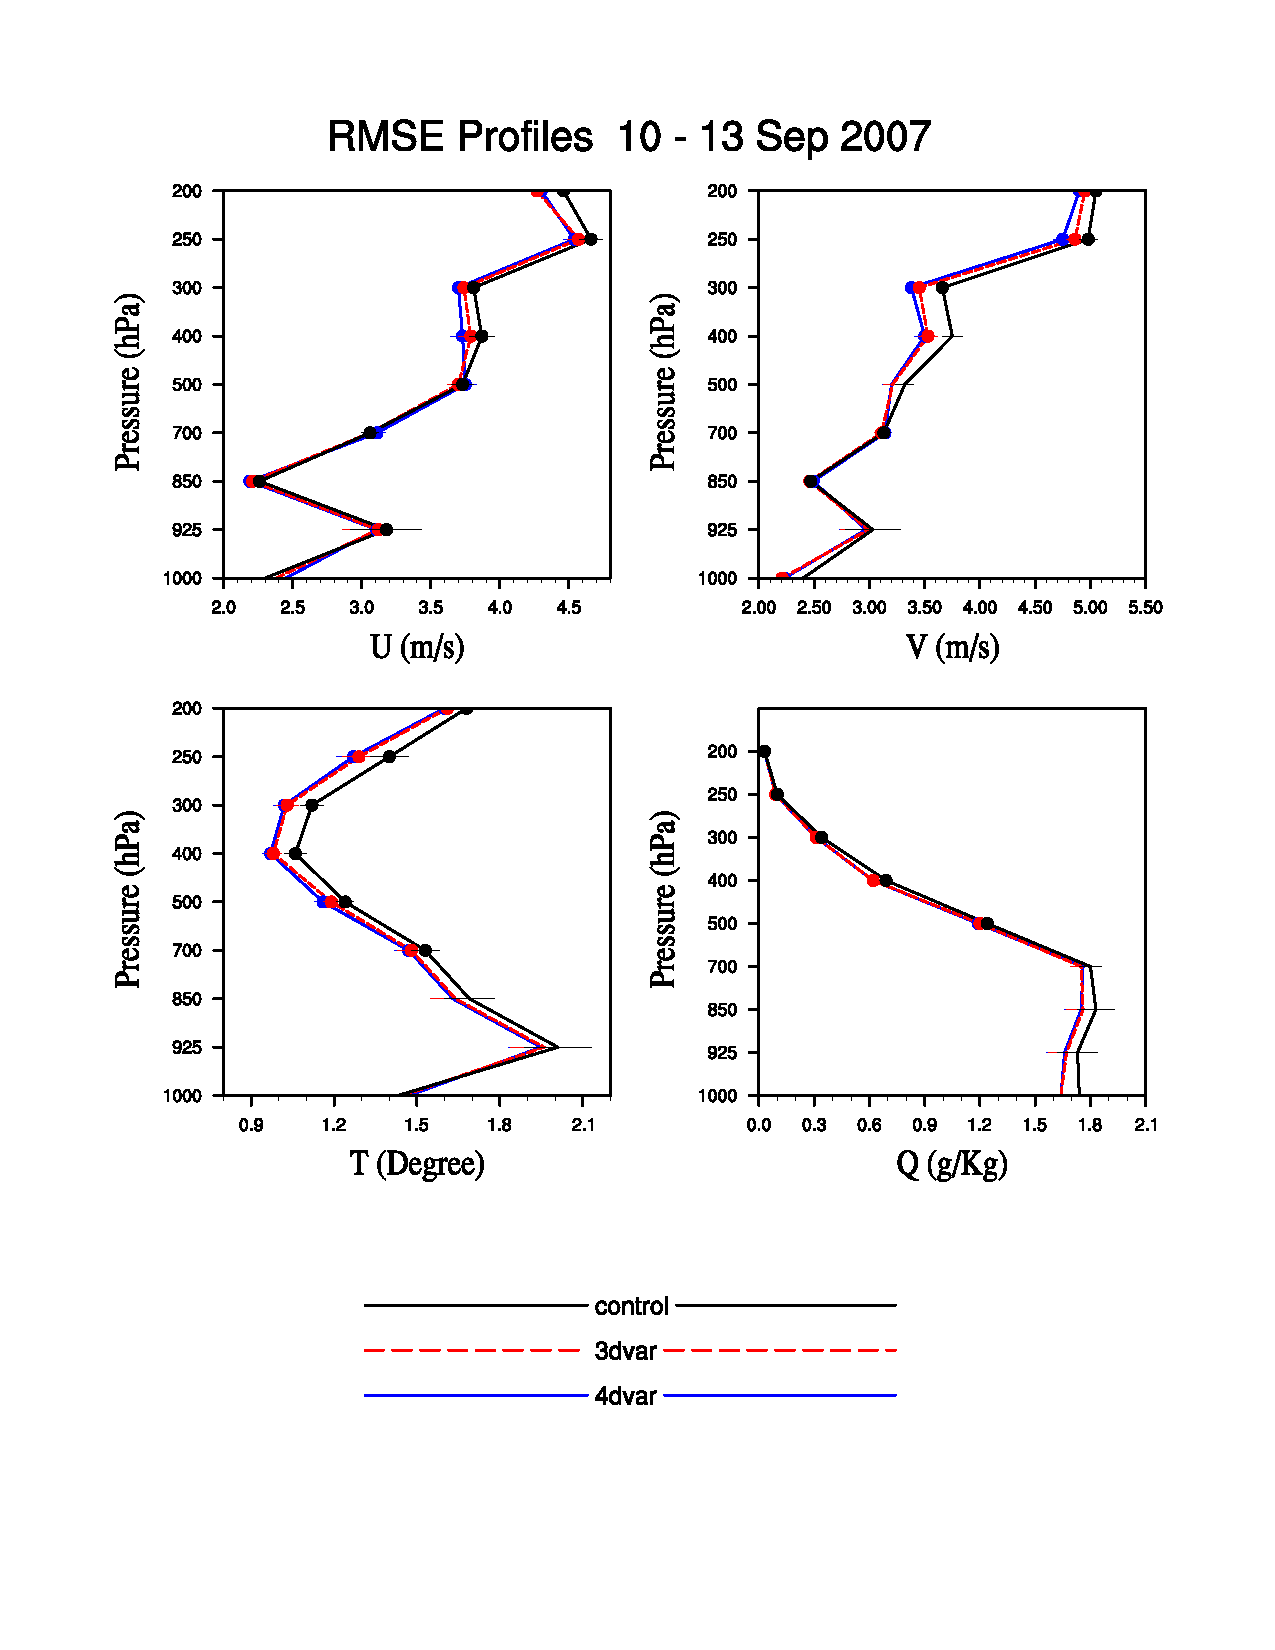
\includegraphics[scale=0.33, trim=0 0 0 80, clip]{Profile_RMSE_24.pdf}
\end{center}
}

\frame{
\frametitle{RMSE Verification---30h}
\begin{center}
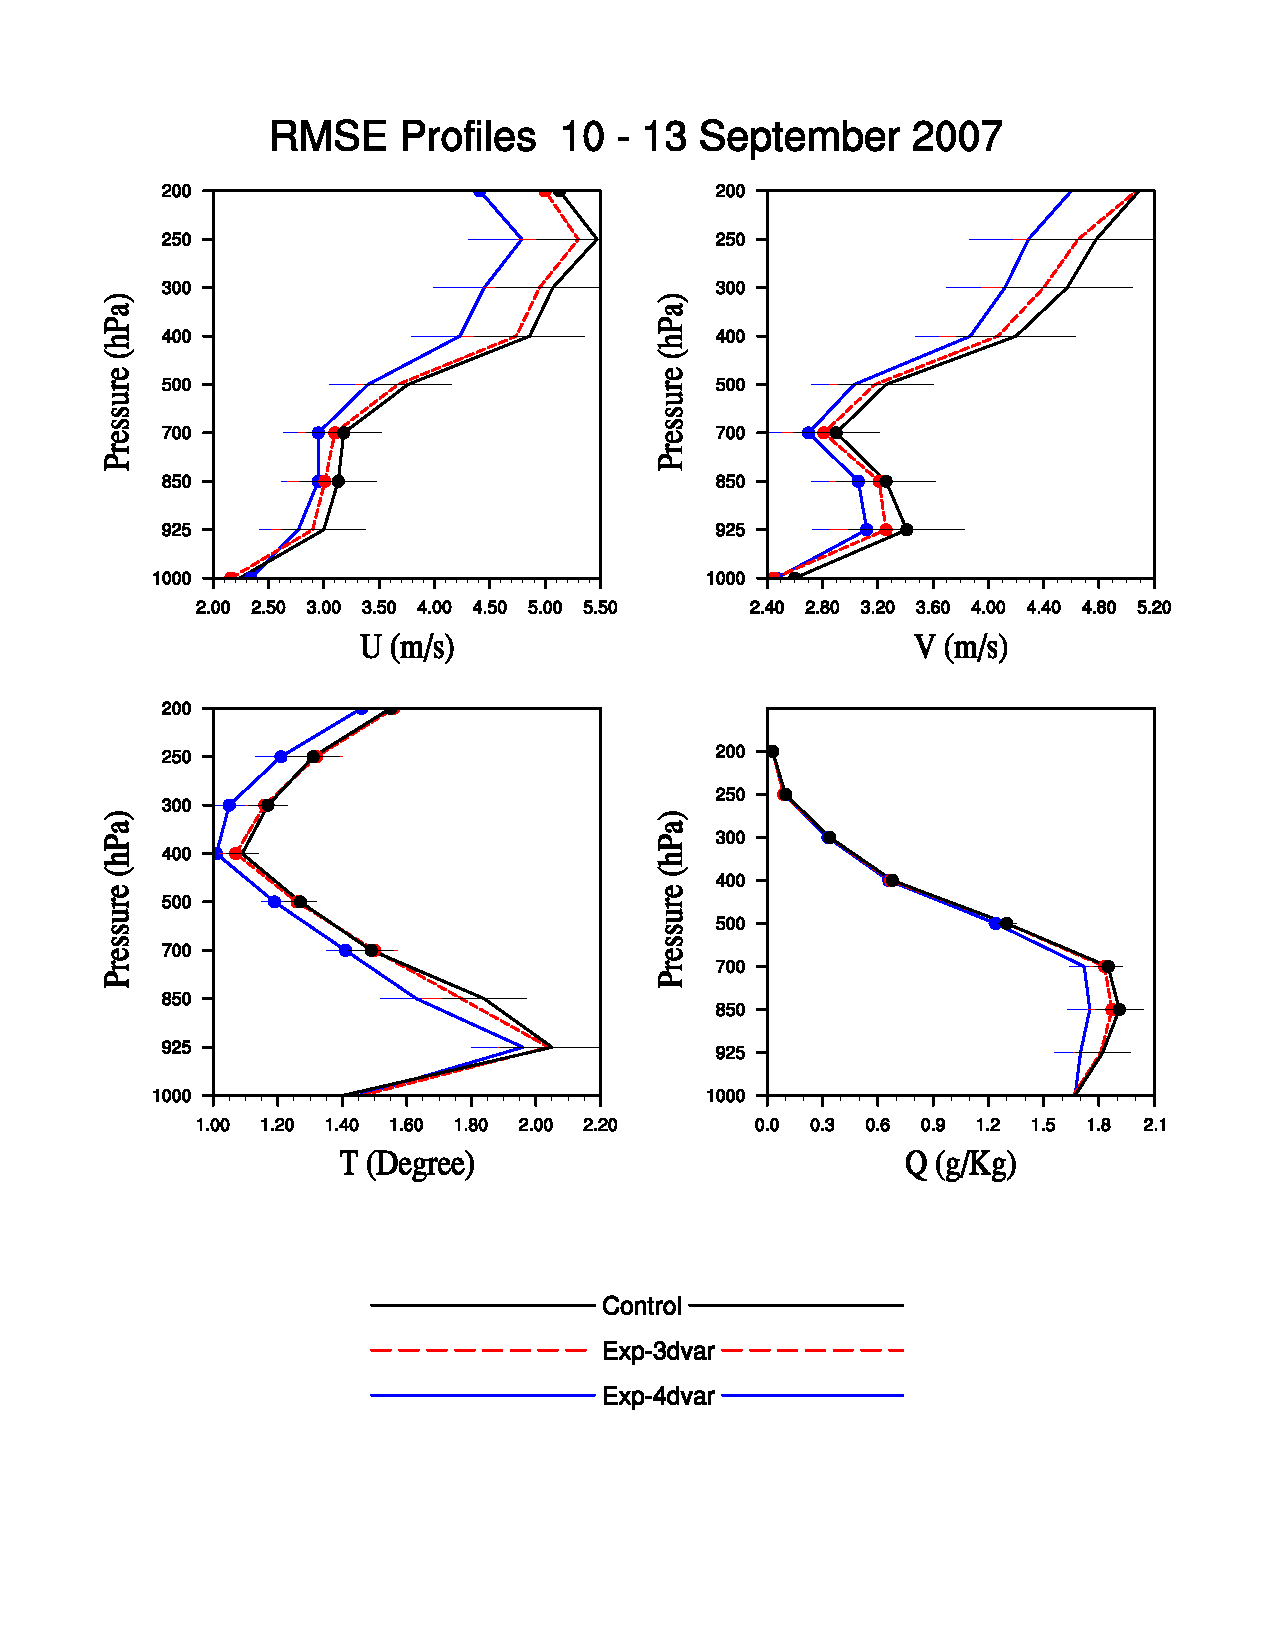
\includegraphics[scale=0.33, trim=0 0 0 80, clip]{Profile_RMSE_30.pdf}
\end{center}
}

\frame{
\frametitle{RMSE Verification---36h}
\begin{center}
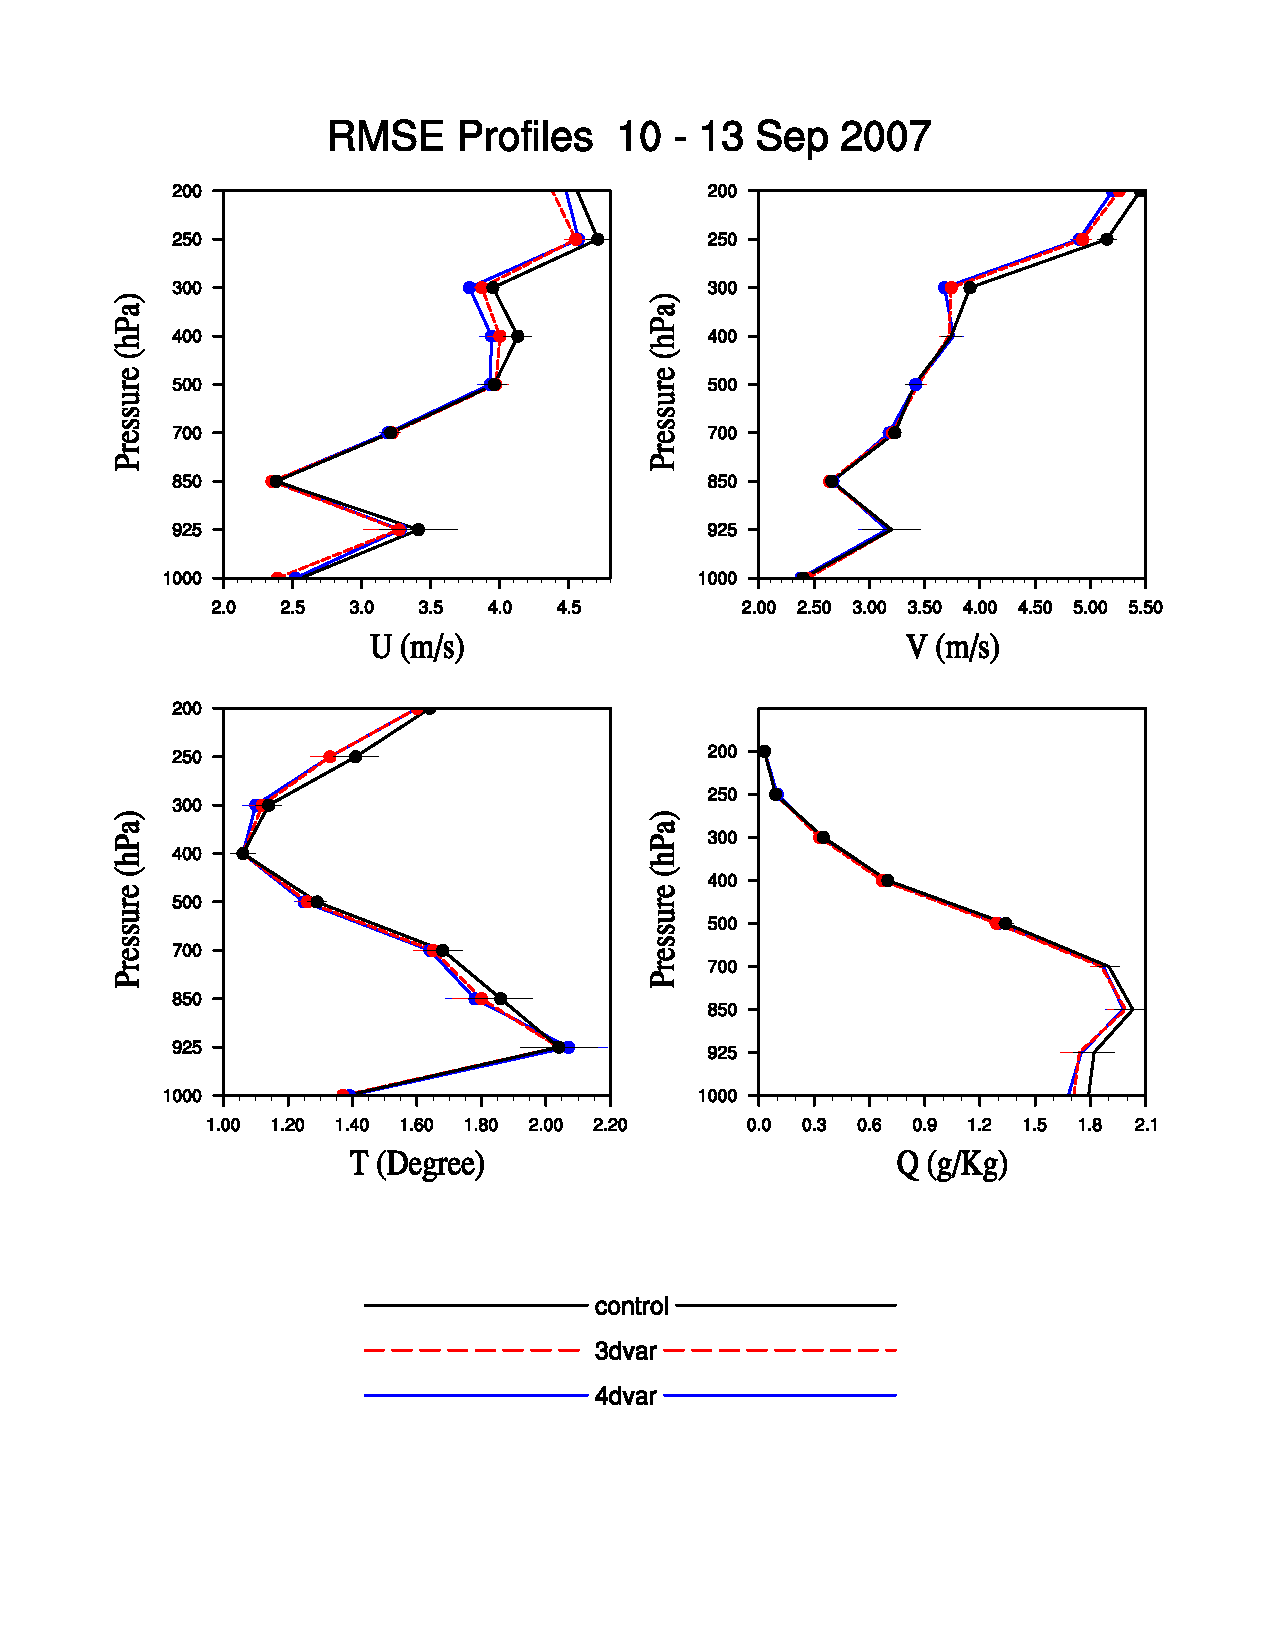
\includegraphics[scale=0.33, trim=0 0 0 80, clip]{Profile_RMSE_36.pdf}
\end{center}
}

\frame{
\frametitle{RMSE Verification---42h}
\begin{center}
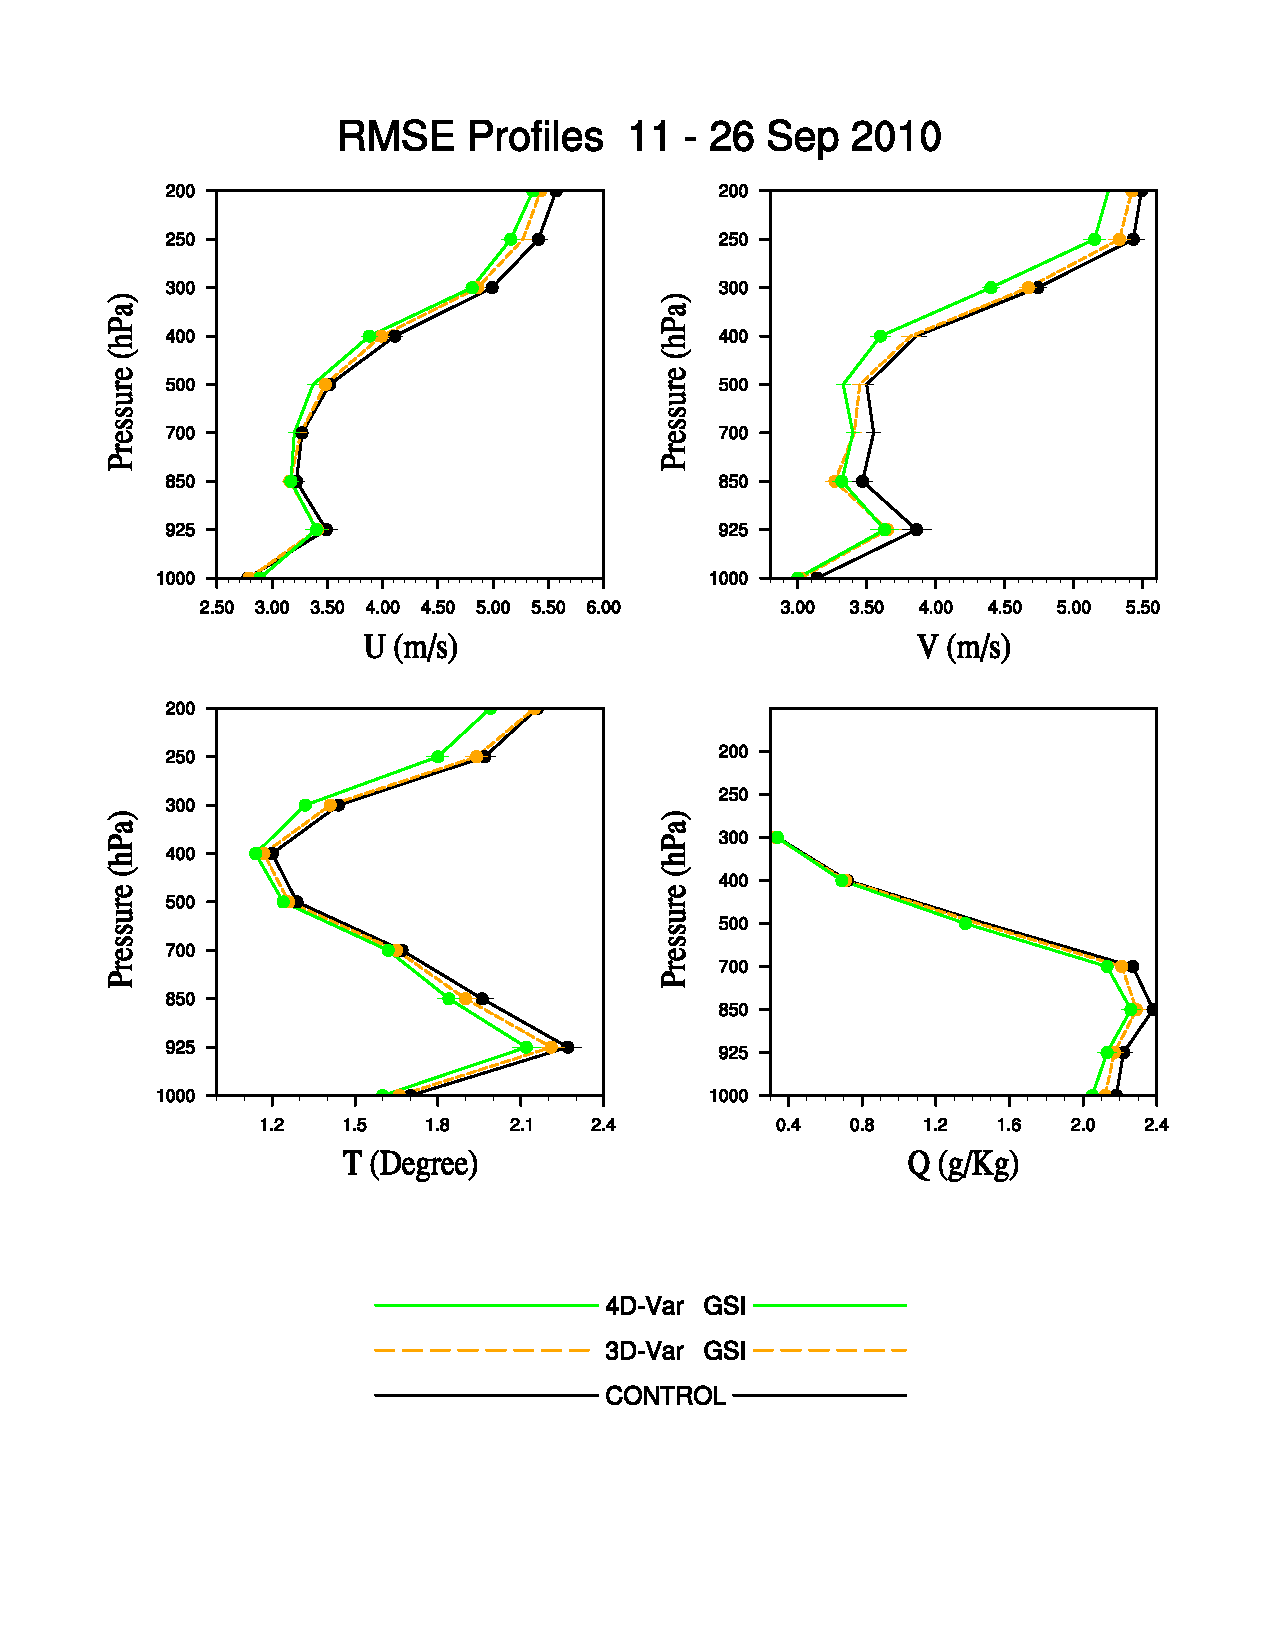
\includegraphics[scale=0.33, trim=0 0 0 80, clip]{Profile_RMSE_42.pdf}
\end{center}
}

\frame{
\frametitle{RMSE Verification---48h}
\begin{center}
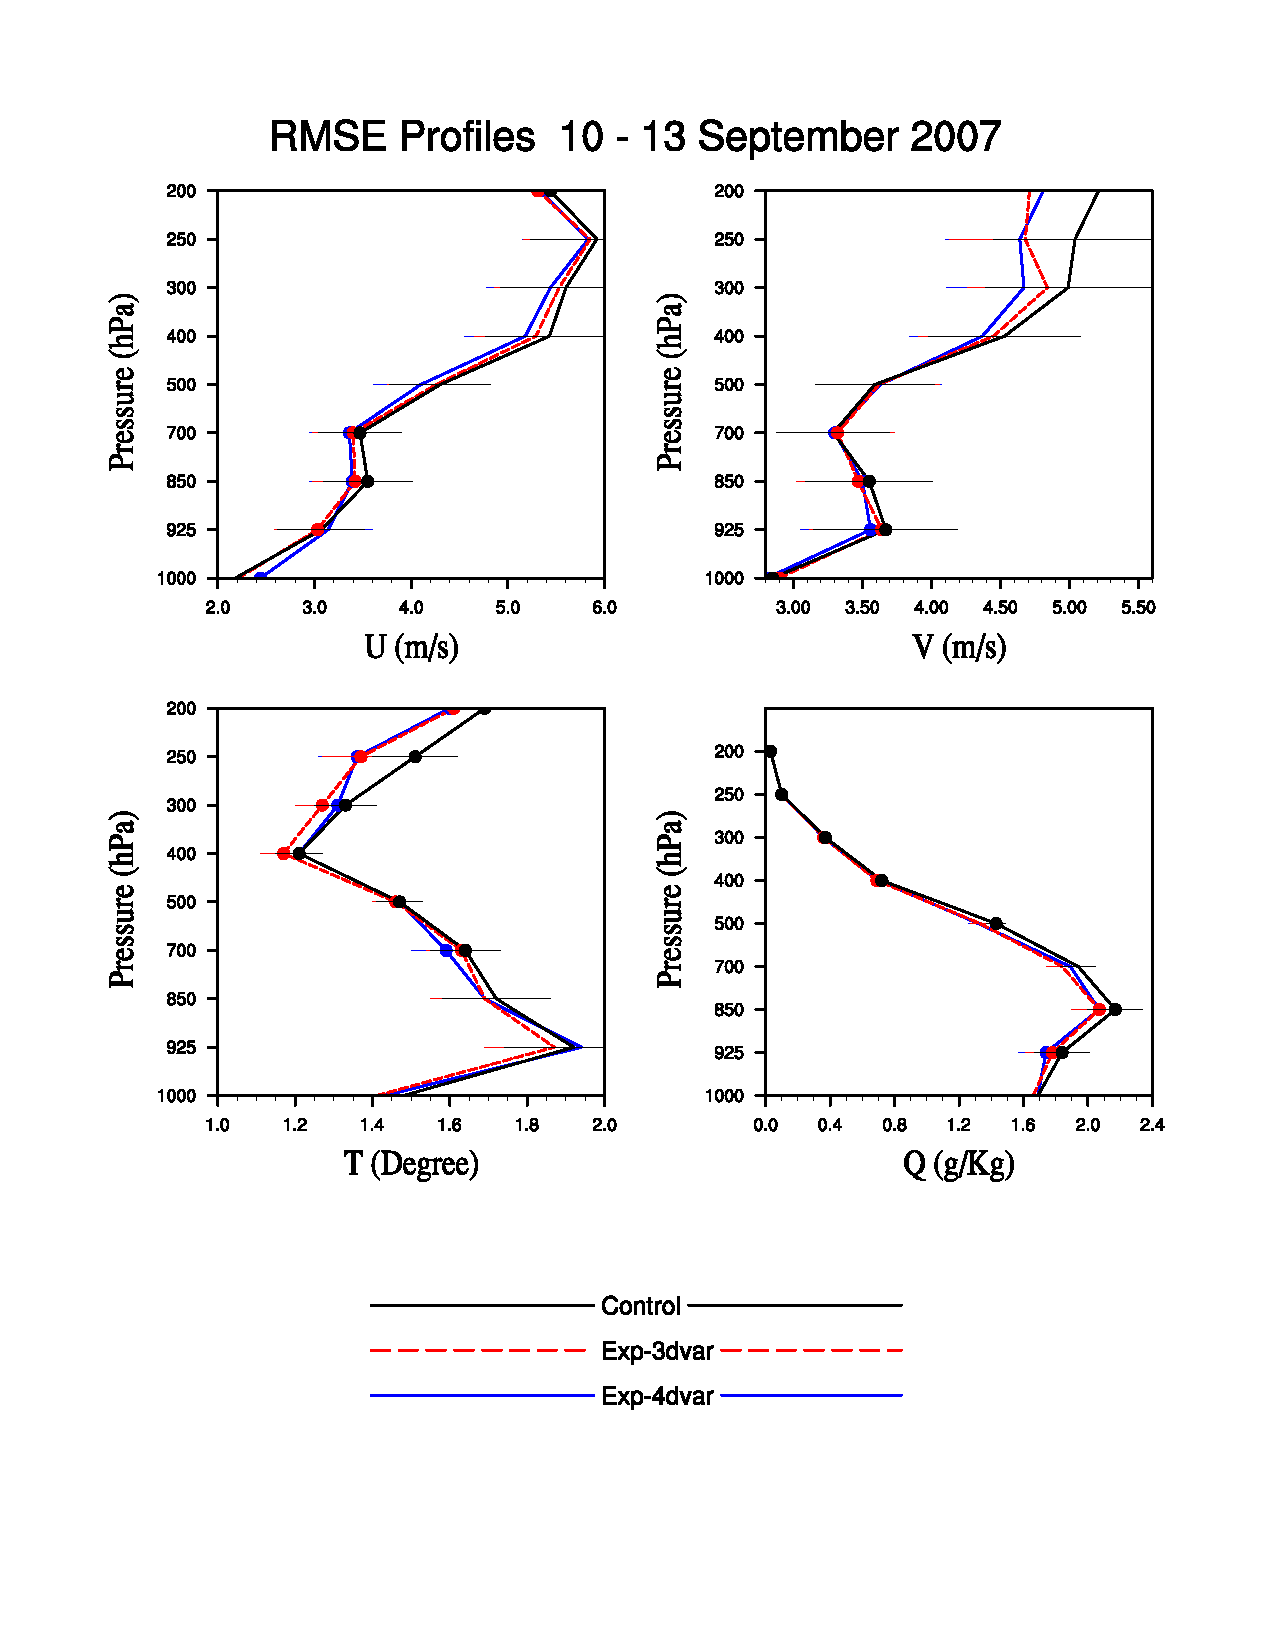
\includegraphics[scale=0.33, trim=0 0 0 80, clip]{Profile_RMSE_48.pdf}
\end{center}
}

%%%%%%%%%%%%%%%%%%%%%%%%%%%%%%%%%
\section{Summary}

\frame{
\frametitle{Summary}
\begin{itemize}
	\item The basic GSI-based WRF 4D-Var system was developed. \pause
	\item The single observation exp.  confirms that the system is valid and is able to produce flow dependent increments. \pause
	\item The increments produced by 4D-Var run with tutorial case are comparable with the 3D-Var run.\pause
	\item The real case shows the desirable performance of 4D-Var.
\end{itemize}
}

\frame{
\frametitle{Latest achievements}
\begin{itemize}
	\item Implementation of the simplified physics packages into WRFPLUSV3 is done: surface drag(bl\_pbl\_physics=98), large scale condensation(mp\_physics=98) and a simplified cumulus scheme(cu\_physics=98). \pause	
	\item Parallelization of WRF tangent linear model is done. 
\end{itemize}
\begin{columns}[c]
\column{6cm}
\begin{center}
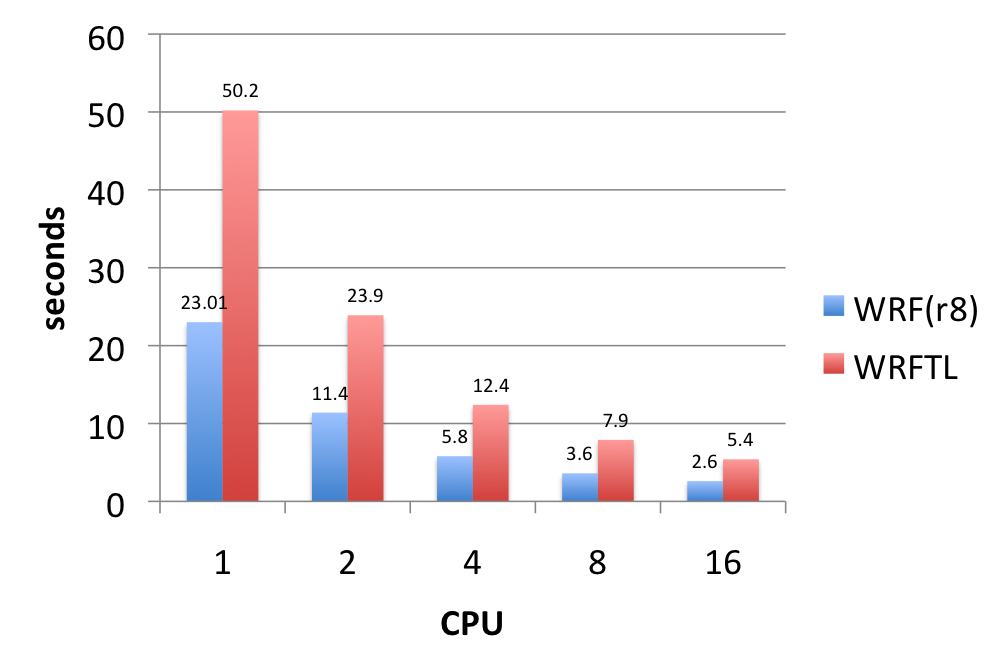
\includegraphics[scale=0.33, trim=0 0 0 0, clip]{wrftl_performance.png}
\end{center}
\column[c]{3.5cm}
\begin{block}{One-time step timing}
\begin{itemize}
	\item \tiny{350x250x57L @27KM, time\_step=150s}
	\item Intel(R) Xeon(R) X7560 @ 2.27GHz
	\item 64G Memory
	\item 8 Processors , 8 cores/processor
	\item PGI 8.0-4 64-bit compiler.
\end{itemize}
\end{block}
\end{columns}
}


%%%%%%%%%%%%%%%%%%%%%%%%%%%%%%%%%%%
\frame{
\begin{center}
~\\
~\\
~\\
~\\
~\\
{\huge{\color{red}Thank You}}\\
~\\
~\\
~\\
~\\
~\\
{\tiny{\color{blue}The NESL Mission is: \\
To advance understanding of weather, climate, atmospheric composition and processes;\\
To provide facility support to the wider community; and, \\
To apply the results to benefit society.\\}}
~\\
{\small{NCAR is sponsored by the National Science Foundation}}
\end{center}
}

\end{document}
